%versi 2 (8-10-2016)
\chapter{Landasan Teori}
\label{chap:teori}

\section{Tanah sawah}
\label{sec:skripsi} 
  Tanah sawah merupakan kata majemuk yang dihasilkan dari penggabungan dua suku kata, tanah dan sawah. Berdasarkan KBBI (Kamus Besar Bahasa Indonesia), tanah dapat diartikan sebagai bahan-bahan dari bumi; bumi sebagai bahan sesuatu, sedangkan sawah dapat diartikan sebagai tanah yang digarap dan diairi untuk tempat menanam padi. Secara umum, tanah sawah dapat didefinisikan sebagai lahan tanah yang dikelola untuk bercocok tanam tanaman padi. Berbagai jenis tanah dapat disawahkan, namun kebutuhan tanaman untuk hidup tetap harus terpenuhi, seperti kadar air yang memadai \cite{pujiarti:18:sawah}. 
  
%\dtext{11-12} 

\subsection{Klasifikasi tanah sawah}
\label{sec:latex}

Tanah kering yang diberi air atau tanah rawa yang "dikeringkan" dengan membuat saluran drainase dapat menjadi tanah sawah. Sawah dapat diklasifikasikan berdasarkan asal air yang diterimanya. Sawah yang menerima air dari hasil irigasi disebut dengan sawah irigasi, sedangkan yang menerima dari air hujan disebut dengan sawah tadah hujan. Sawah pasang surut dapat ditemukan di daerah pasang surut, begitupula sawah lebak yang dikembangkan di daerah rawa-rawa lebak\footnote{\url{http://balittanah.litbang.pertanian.go.id/ind/dokumentasi/buku/tanahsawah/tanahsawah1.pdf}}\cite{luh:07:kualitastanah}.

\begin{enumerate}
\item{Sawah irigasi}

Sawah irigasi adalah sawah yang menggunakan sistem pengairan (pengelolaan air) yang berasal dari bendungan atau waduk secara teratur. Dengan sistem pengairan yang diatur secara teknis, maka air yang dibutuhkan untuk menjaga kondisi tanah sawah tidak bergantung pada curah hujan. Hal ini disebabkan pengairan tersebut dapat diperoleh dari sungai, waduk atau bendungan.
Sawah irigasi menggunakan air terbesar dibandingkan jenis sawah lainnya, hal ini menyebabkan sebanyak 85\% sawah beririgasi masih dihadapkan kepada masalah efisiensi. Masalah ini disebabkan oleh hilangnya air selama proses irigasi (\textit{distribution  losses}) maupun proses pemakaian (\textit{field  applicationlosses})\footnote{\url{https://dosenpertanian.com/sawah-irigasi/}}. 

\item{Sawah tadah hujan}

Sawah tadah hujan adalah sawah yang memanfaatkan air hujan sebagai sumber utama sistem pengolaan air untuk lahan pertanian. Sistem pengairan sawah tanah hujan bekerja dengan cara menampung air hujan. Hal ini menyebabkan lahan sawah tadah hujan sangat berisiko terkena kekeringan saat musim kemarau tiba. Sawah tadah hujan juga memiliki tingkat kesuburan yang rendah. Tingkat kesuburan sawah tadah yang rendah disebabkan oleh bergantungnya pada curah hujan dan rentannya lahan sawah terhadap serangan hama penyakit. 

\item{Sawah bencah atau sawah pasang surut}

Sawah pasang surut adalah sawah yang umumnya dapat ditemukan disekitar muara sungai dan rawa dekat pantai. Jenis sawah ini hanya dapat diolah satu kali dalam setahun, dan keperluan air untuk tanaman padi dipengaruhi oleh pasang surut air laut. Tanah sawah pasang surut merupakan sebagian dari hasil sedimentasi lumpur, yang dibentuk oleh luapan air sungai saat air laut pasang.

\item{Sawah lebak}

Sawah lebak memiliki kemiripan dengan sawah pasang surut. Sawah lebak umumnya terletak didataran rendah sekitar sungai, untuk ditanamani berbagai macam tanaman padi. Letaknya lahan sawah yang berdekatan dengan sungai, mengakibatkan rawannya tanaman padi terhadap banjir pada musim hujan. Hal ini yang menyebabkannya cukup seringnya lahan sawah lebah dialihfungsikan menjadi lahan perkebunan. 

Perbedaan yang signifikan antara sawah lebak dengan sawah pasang surut adalah sumber utama sistem pengairan yang didapatkan. Sawah pasang surut mengandalkan pasang surut air laut sebagai pemasokan kebutuhan air lahan sawah, sedangkan sawah lebak mengandalkan air hujan sebagai sumber utama sistem pengelolaan air lahan pertanian. Sehingga resiko kekeringan pada sawah tadah hujan juga dapat terjadi pada lahan sawah lebak. 
\end{enumerate}

\subsection{Variabel yang mempengaruhi kondisi tanah sawah}
Tanah yang subur dan memiliki kandungan organik yang cukup, sangat mempengaruhi pertumbuhan dan perkembangan tanaman padi. Untuk mencapai kondisi tanah sawah yang baik maka perlu diketahui variabel yang mempengaruhi kondisi tanah. Variabel yang mempengaruhi kondisi tanah sawah antara lain tingkat keasaaman tanah(pH), tingkat kelembaban tanah, dan suhu tanah serta persawaan.

\begin{enumerate}

    \item{Kadar keasaman tanah (pH)}
    
    pH tanah adalah kadar tingkat keasaaman atau kebasaan suatu tanah yang dapat diukur dengan skala pH antara 0 sampai 14. Jika angka skala pH dari tanah yang diuji menunjukan nilai kurang dari 7, maka tanah yang diuji bersifat asam. Sedangkan tanah yang memiliki nilai pH lebih dari 7 merupakan tanah bersifat basa.
    
    Tanah dengan tingkat keasaman yang tinggi, unsur kalsium, magnesium, dan fosfor akan terikat secara kimiawi. Hal ini menyebabkan tanaman tidak dapat menyerap unsur-unsur tersebut. Kondisi tesebut dapat mengakibatkan tanaman tidak tumbuh secara optimal dan menghasilkan produktifitas yang rendah. Untuk menyesuaikan nilai pH tanah, penggunaan dolomit dengan dosis tertentu dapat diberikan dengan dosis yang sesuai kebutuhan\footnote{\url{https://mitalom.com/pengaruh-derajat-keasaman-tanah-ph-terhadap-tanaman/}}\cite{dariska:01:phtanah}.
    
    
    \item{Tingkat kelembaban tanah}
    
    Komponen mikro yang mempengaruhi kondisi tanah sawah, dan pertumbuhan tanaman padi sangat dipengaruhi oleh kelembaban tanah. Kelembaban yang berlebihan dapat menimbulkan penyerapan air yang berlebihan oleh akar tanaman yang berakibat pada busuknya tanaman, sedangkan kekurangan kelembaban dapat menimbukan pertumbuhan tanaman yang tidak optimal karena kurangnya air untuk kebutuhan tanaman. Setiap jenis tanaman memiliki tingkat kelembaban tanah ideal yang berbeda-beda. Kelembaban tanah juga mempengaruhi aktivitas mikroorganisme dalam tanah dan ketersediaan unsur hara\cite{chusnul:01:kelembabantanah}.
     
    \item{Suhu tanah persawahan}
    
    Aktivitas biologi tanah seperti organisme tanah, sangat dipengaruhi oleh temperatur tanah. Proses penguraian bahan organik, reaksi kimia, dan bahan induk tanah juga sangat dipengaruhi oleh suhu tanah. Proses pertumbuhan tanaman padi juga dipengaruhi oleh suhu tanah melalui tingkat kelembaban tanah. Suhu dalam tanah dapat berubah-ubah (fluktuasi), bergantung pada perubahan sumber energi, waktu dan tingkat kedalaman tanah. Temperatur tanah dipagi hari relatif lebih kecil dibandingkan disiang hari. Hal ini disebabkan oleh pancaran radiasi matahari yang diterima oleh permukaan tanah lebih besar pada siang hari. 
    
    Suhu tanah juga berbeda-beda bergantung pada tingkat kedalaman tanah (10cm, 20cm, dan 30cm). Semakin dalam tanah, maka semakin rendah suhunya. Perbedaan suhu ini dipengaruhi oleh transfer panas dari pancaran radiasi matahari, yang belum mencapai kedalaman tertentu. Transfer panas yang dipancarkan radiasi matahari dirambatkan ke lapisan tanah yang lebih dalam secara konduksi. Faktor lain yang mempengaruhi perubahan suhu tanah adalah sumber energi panas yang diterima dari matahari. Perubahan suhu ini dipengaruhi oleh iklim cuaca, keadaan tanah dan bentuk topografi (bentuk permukaaan tanah)\footnote{\url{https://www.slideshare.net/iqrimhayamada/suhu-tanah}}.

\end{enumerate}

%\dtext{13-14}


\subsection{Klasifikasi kondisi tanah sawah}
\label{sec:template}
Untuk mengetahui kondisi tanah sawah maka diperlukan pengukuran variable yang mempengaruhi kondisi tanah sawah seperti kadar keasamaan tanah sawah(pH), tingkat kelembaban tanah, dan suhu tanah. Tanaman padi memiliki nilai ideal tertentu untuk masing-masing variabel, bergantung dari jenis tanah sawahnya. 

Nilai keasaman tanah sawah(pH) yang ideal untuk tanaman padi adalah 7, yang mengindikasikan bahwa tanah sawah bersifat netral, tidak asam maupun basa. Namun, beberapa jenis tanaman padi masih dapat tumbuh dan berkembang pada tanah dengan pH yang asam, dengan tingkat toleransi nilai pH maksimal 5. 

Selain kadar keasaman, variabel lain yang mempengaruhi pertumbuhan tanaman padi adalah kelembaban. Berdasarkan pengukuran yang dilakukan menggunakan metode SRI  (\textit{System of Rice Intensification}) dan model Algoritma Genetika, didapatkan hasil kelembaban tanah optimum untuk tanaman padi adalah 0.622 (basah) atau setara dengan 62\%\footnote{\url{https://repository.ipb.ac.id/bitstream/handle/123456789/69941/JI2014-Vol9\%2cNo1.pdf?sequence=1&isAllowed=y}}. Namun, hal ini tidak berlaku untuk semua jenis tanaman. Tingkat kelembaban yang dibutuhkan untuk setiap tanaman berbeda-beda, sebagaimana yang diperlihatkan pada Tabel~\ref{tab:Tabel kelembaban ideal tanaman} berikut.

\begin{table}[H] 
	\centering 
	\caption{Tabel kelembaban ideal tanaman}
	\label{tab:Tabel kelembaban ideal tanaman}
	\begin{tabular}{cccc}
		\toprule
		 Jenis tanaman & Kelembaban ideal & Jenis tanaman & Kelembaban ideal  \\

		\midrule
		Tomat & 40\%-60\%  & Kubis & 40\%-60\% \\
        Terong & 40\%-60\% & Bawang & 30\%-50\% \\
        Kacang tanah & 30\%-50\% & Kentang & 30\%-50 \% \\
        Mentimun & 50\%-70\% & Bunga kol & 40\%-60 \% \\
        Wortel & 30\%-50\% & Buah-buahan & 30\%-50 \% \\
        Seledri & 40\%-60\% & Cabai & 40\%-60 \% \\

		\bottomrule
		
	\end{tabular} 
\end{table}

Suhu merupakan salah satu faktor lain yang mempengaruhi pertumbuhan tanaman padi. Pada dataran rendah suhu udara yang ideal untuk tanaman padi adalah sekitar 22$^{\circ}$C sampai 26$^{\circ}$C, sedangkan untuk dataran tinggi suhu udara yang ideal adalah sekitar 18$^{\circ}$C sampai 22,5$^{\circ}$C. Suhu tanah yang kurang dari 10$^{\circ}$C akan menghambat perkembangan mikroba tanah dan menghambat penyerapan hara oleh tanah. Sedangkan suhu yang melebihi 40$^{\circ}$C akan menyebabkan mikroba dalam tanah menjadi tidak aktif, kecuali untuk mikroorganisme tertentu. Pada umumnya, tingkat aktivitas optimum dari organisme tanah memerlukan suhu tanah sekitar 18$^{\circ}$C sampai 30$^{\circ}$C\footnote{\url{https://www.slideshare.net/iqrimhayamada/suhu-tanah}}.
%\dtext{15-16}


\subsection{Metode pemantauan kualitas tanah sawah}
Terdapat beberapa cara untuk melakukan pemantauan kualitas tanah sawah. Metode yang masih sering dilakukan adalah \textit{sampling} atau pemanfaatan IoT (Internet of Things). Perbedaan kedua metode ini terletak pada biaya, waktu, dan tempat. Pemantauan yang dilakukan dengan melakukan pengujian kondisi tanah sawah menggunakan metode \textit{sampling} memiliki ketepatan yang lebih akurat, namun membutuhkan waktu yang lebih lama dan biaya yang lebih mahal. 
\begin{itemize}
    \item \textit{Sampling}
    
    \textit{Sampling} adalah proses pengambilan atau memilih n buah elemen dari populasi yang berukuran N (Lohr, 1999). \textit{Sampling} dalam pemantauan kualitas tanah dilakukan dengan cara mengambil tanah sawah yang diteliti menggunakan ring sampel, bor, dan pisau lapang. Tanah sawah yang dijadikan \textit{sampling} akan dibawa ke Labotarium Tanah dan Lingkungan untuk diuji kualitasnya. Uji labotarium dilakukan menggunakan metode tertentu kualitas tanah ditetapkan dengan metode yang disajikan seperti Tabel~\ref{tab:Parameter dan Metode Analisis Kualitas Tanah} \footnote{\url{https://simdos.unud.ac.id/uploads/file_penelitian_1_dir/bbc895c97c05ccd2a106b91f9843705b.pdf}}.
    
    \begin{table}[H] 
	\centering 
	\caption{Parameter dan Metode Analisis Kualitas Tanah (Lal,1994)}
	\label{tab:Parameter dan Metode Analisis Kualitas Tanah}
	\begin{tabular}{ccc}
		\toprule
		 Parameter & Satuan & Metode \\

		\midrule
		Sifat Fisik\\
		\hline
		Kadar Air Tanah & \% & Gravimetri\\
		Tekstur Tanah & \% & Metode Pipet\\
		Berat Volume (bulk density) & g/cm$^3$ & Ring sampler \\
		Porositas & \% & Ring sampler\\
		\hline
		Sifat Kimia\\
		\hline
		pH &  & Potensiometri H$_2$O 1:2,5\\
		N-Total & \% & Destilasi Makro Kjeldahl\\
		P - Tersedia & mg/kg & Bray-1\\
		K - Tersedia & mg/kg & Bray-1\\
		KTK & me/100g & Ekstraksi NH$_4$OAc 1 N pH 7\\
		KB - Tersedia & \% & Ekstraksi NH$_4$OAc 1 N pH 7\\
        \hline
		Sifat Biologi\\
		\hline
		C-organik & \% & Walkley \& Black\\
		Total Mikroba & cfu/g tanah mg C-C$_o2$ & Plate Count\\
		Respirasi & mg C-CO$_2$/kg & Evolusi CO$_2$\\
		C-biomassa & mg CO$_2$/kg & Simulasi Respirasi\\
		

		\bottomrule
		
	\end{tabular} 
\end{table}
    
    \item Pemanfaatan IoT (\textit{Internet of Things})
    
    Perkembangan teknologi yang begitu pesat membantu berbagai jenis penelitian, termasuk pemantauan kondisi tanah sawah. Pemanfaatan Iot untuk pemantaukan kualitas tanah sawah sudah cukup sering dilakukan terutama di Indonesia. Aplikasi berbasis android maupun desktop yang terintegrasi dengan sensor yang disebar di area persawahan, membantu para petani dalam mendapatkan informasi tanah sawah yang mereka kelola. Pemanfaatan IoT memungkinkan pengguna untuk mendapatkan data secara \textit{real-time} dan tanpa perlu mengeluarkan biaya yang mahal. Namun data yang didapatkan tidak akan seakurat metode \textit{sampling} yang diuji di labotarium.
    
\end{itemize}

\section{WSN (\textit{Wireless Sensor Network})}  
WSN (\textit{Wireless Sensor Network}) merupakan jaringan sensor nirkabel yang mengacu pada sekumpulan node sensor yang saling terhubung. Node sensor akan disebar dalam bentuk spasial pada area yang ingin dilakukan pengukuran atau \textit{sensing}. WSN juga berguna untuk memantau hasil sensing kondisi suatu lingkungan yang dilakukan oleh sensor. Selain itu WSN juga dapat mengatur data yang akan dikirimkan dan dikumpulkan di \textit{base station}.
Setiap node sensor memiliki radio \textit{transceiver} yang digunakan untuk berkomunikasi dan mengirimkan data ke lokasi pusat. Bentuk radio \textit{transceiver} untuk setiap node menggunakan antena internal ataupun anterna eksternal.

\subsection{Pemanfaatan \textit{Wireless Sensor Network}}
Saat ini, teknologi WSN tidak hanya dimanfaatkan untuk keperluan ilmu komputasi saja. Penggunaan teknologi WSN telah digunakan untuk melakukan pemantauan ataupun pengukuran, diberbagai bidang ilmu pengetahuan. Selain digunakan untuk membantu penelitian di bidang ilmu pengetahuan, teknologi WSN juga dimanfaatkan oleh pihak militer dan industri.

\begin{enumerate}
    \item Bidang Kesehatan
    
    Pemanfaatan WSN di bidang kesehatan telah banyak diterapkan. Beberapa penerapan WSN di bidang kesehatan adalah pemanfaatan IoT (\textit{Internet of Things}) untuk perangkat medis untuk mendeteksi kondisi tubuh manusia. Selain itu, WSN juga dimanfaatkan untuk melakukan pemantauan dan diagnosa kesehatan pasien secara \textit{real-time}.
    
    \item Pemantauan Lingkungan
    
    Untuk pemantauan lingkungan, WSN memiliki banyak pengaplikasian yang berbeda di berbagai jenis lingkungan. Beberapa contoh pemanfaatan WSN untuk pemantauan lingkungan antara lain, pemantauan polusi udara, mendeteksi kebakaran hutan, mendeteksi longsor, mendeteksi ancaman bencana alam, dan lain-lain.  
    
    \item Bidang Agrikultur
    
    Di bidang agrikultur WSN digunakan untuk meningkatkan produktivitas hasil panen. Penerapan WSN dapat dilakukan untuk melakukan pengamatan, pengukurann, dan respon terhadap variable tanah. Pemantauan tersebut bertujuan untuk meningkatkan ataupun menjaga kualitas hasil panen, dari pemanfaatan data lingkungan pertanian. 
    
    
    \item Bidang Infrastruktur
    
    \textit{Wireless sensor network} juga digunakan dalam pembangunan infrastruktur. Pemanfaatan WSN biasa digunakan untuk melakukan pengamatan kondisi pembangunan infrastruktur, baik dari segi bangunan maupun geografis. Penerapan WSN untuk membantu pembangunan infrastruktur dilakukan secara berkala dan \textit{real-time} untuk menjaga kondisi lingkungan selama pemabangunan.
    
    \item Bidang Militer
    
    Salah satu contoh pemanfaatan WSN di bidang militer adalah Wide Area Tracking System (WATS). WATS merupakan prototipe jaringan yang mengunakan teknologi WSN untuk mendeteksi ancaman nuklir. Pemanfaatan WSN lainnya di bidang militer adalah peluru kendali, yang memiliki sistem pengendali otomatis untuk mencari sasaran berdasarkan suhu temperatur.
    
    \item Bidang Planologi
    
    Dibidang planologi, salah satu pemanfaatan WSN digunakan untuk memantau jumlah kendaraan pada suatu area untuk mengatasi masalah kemacetan, ataupun membantu proyek rekayasa arus lalu-lintas. Pemanfaatan WSN memungkinkan pengiriman informasi jumlah kendaraan secara \textit{real-time} ke pengguna. 
    
    \item Bidang Industri
    
    Pemanfaatan WSN di bidang industri cukup beragam, bergantung jenis barang yang diproduksinya. Untuk industri otomotif, penggunaan WSN digunakan sebagai fitur keamanan ataupun kenyamanan. Salah satu pemanfaatannya adalah untuk mendeteksi lingkungan sekitar kendaraan, untuk mencegah terjadinya benturan yang disebabkan oleh \textit{blind-spot}.
    
\end{enumerate}

\subsection{Klasifikasi Node}
 Titik komunikasi atau titik distribusi komunikasi yang saling terhubung dapat didefinisikan sebagai node. Dari sudut pandang jaringan, node dapat didefinisikan sebagai anggota jaringan yang dapat saling berkomunikasi untuk menerima atau menghasilkan data, ataupun keduanya\footnote{\url{https://www.nesabamedia.com/pengertian-node/}}.
Pada \textit{Wireless Sensor Network} terdapat 3 jenis node yang memiliki karakteristik dan fungsional yang berbeda. Variasi node yang terdapat pada WSN antara lain node sensor, router, dan sink node (\textit{base station}).
\begin{enumerate}
    \item Node Sensor
    
    Node sensor adalah node dalam jaringan yang digunakan untuk melakukan pemrosesan, pengumpulan informasi yang didapatkan dari hasil \textit{sensing}, dan berkomunikasi dengan node lain yang terhubung dalam jaringan. Node sensor juga berfungsi untuk melakukan pengukuran kondisi suatu lingkungan berdasarkan hasil \textit{sensing} yang diterimanya untuk dikirimkan ke \textit{gateway}.
    
    \item Router
    
    Router adalah node yang menjadi perantara antara node sensor dengan node sensor lainnya, agar node dapat saling berkomunikasi. Router dapat menerima paket yang didapatkan dari suatu node untuk diteruskan ke node lain.
    
    \item Sink Node
    
    Sink node atau \textit{Base station} adalah komponen WSN yang bertindak  (\textit{attach}) sebagai \textit{gateway} antara node sensor dengan \textit{notebook}. \textit{Base station} juga merupakan bagian terakhir dari rangkaian WSN yang berfungsi untuk meneruskan data hasil sensing node sensor ke \textit{notebook} atau server. Untuk perangkat keras arduino, komponen yang digunakan sebagai \textit{base station} adalah Raspberry.
    
\end{enumerate}


\subsection{Komponen Node Sensor}

Node sensor terdiri dari komponen-komponen yang saling terhubung dengan fungsionalnya masing-masing. Komponen utama node sensor antara lain \textit{controller}, \textit{transceiver}, \textit{memory}, \textit{power source}, dan sensor.

\begin{itemize}
    \item \textit{Controller}
    
    \textit{Controller} bertindak sebagai pengontrol fungsionalitas komponen-komponen lain pada node sensor. Selain itu, \textit{controller} juga memiliki tugas untuk memproses data. Mikrokontroler menjadi alternatif yang paling umum digunakan untuk melakukan pemrosesan pada node sensor. Hal ini dikarenakan mikirokontroler lebih mudah untuk dihubungkan dengan perangkat lain. Mikrokontroler juga menggunakan konsumsi daya yang lebih rendah dan biaya yang lebih murah.
    
    \item \textit{Transceiver}
    
    Transceiver adalah perangkat yang digunakan untuk menerima dan memancarkan sinyal dalam jaringan. Dengan \textit{transceiver}, node sensor dapat terhubung dengan jaringan dan berkomunikasi dengan node sensor lainnya. Teknologi yang umum digunakan untuk terhubung dalam jaringan adalah \textit{baseband}.
    
    \item \textit{Memory}
    
    RAM (Random Access Memory) merupakan perangkat \textit{volatile} yang digunakan sebagai tempat penyimpanan data sementara. Data yang diterima dari hasil \textit{sensing} oleh sensor, akan disimpan pada RAM. Namun, penyimpanan ini hanya bersifat sementara, sebelum data tersebut dikirimkan ke \textit{base station}. \textit{Memory} yang terdapat pada node sensor bersifat \textit{volatile}, hal ini dapat mengakibatkan hilangnya data jika node sensor mati. 
    
    \item \textit{Power source}
    
    Energi yang dibutuhkan untuk mengoperasikan fungsionalitas seluruh komponen berasal dari \textit{power source} atau \textit{power supply}. Penyediaan energi ini dapat memiliki dari dua jenis metode, yaitu \textit{storing energy} atau \textit{energy scavenging}. Pada metode \textit{storing energy}, node sensor menggunakan baterai sebagai sumber energi utamanya. Sedangkan pada pendekatan \textit{energy scavenging}, node sensor menggunakan perubahan energi sebagai sumber energi utamanya. Energi pada metode \textit{energy scavenging} didapatkan setelah mengonversi pemanfaatan energi cahaya matahari, angin, ataupun air menjadi listrik untuk mengoperasionalkan node sensor.
    
    \item \textit{Analog to Digital Converter} (ADC)
    
    ADC adalah perangkat kecil berbentuk chip yang berfungsi untuk mengubah sinyal yang dikirimakan oleh sensor dari analog menjadi digital. \textit{Analog to Digital Converter} juga dapat berbentuk suatu modul yang terdiri dari barisan kode yang di \textit{upload} ke node sensor.
    
    \item Sensor
    
    Sensor merupakan perangkat yang digunakan untuk melakukan \textit{sensing} dan pengukuran, terhadap suatu kondisi pada lingkungan yang diamati. Sensor juga dapat merespon terhadap perubahan suatu kodisi lingkungan seperti suhu ataupun kelembaban.
\end{itemize}

Secara umum sebuah node sensor memiliki struktur seperti yang ditunjukkan pada Gambar~\ref{fig:Node sensor}.

    \begin{figure}[H]
    	\centering  
    	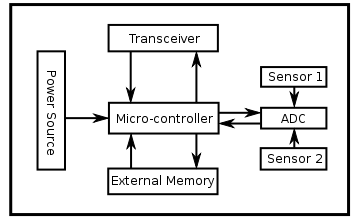
\includegraphics[scale=0.7]{sensor-node.png}  
    	\caption[Node sensor]{Node sensor} 
    	\label{fig:Node sensor} 
    \end{figure} 

\subsection{Arsitektur \textit{Wireless Sensor Network}} \label{Arsitektur WSN}
Arsitektur pada WSN terbagi menjadi dua jenis, yaitu arsitektur \textit{flat} dan arsitektur \textit{hirarkikal}. Perbedaan dua jenis arsitektur ini terdapat pada cara node sensor dalam berkomunikasi. Secara sederhana, pada arsitektur \textit{flat}, node yang disebar dapat langsung mengirimkan data hasil \textit{sensing} ke \textit{base station}. Sedangkan pada arsitektur \textit{hirarkikal}, node yang disebar harus mengirimkan data ke \textit{cluster head} terlebih dahulu, sebelum diteruskan ke \textit{base station} \cite{ivan:20:wsn}.

    \begin{figure}[H]
    	\centering  
    	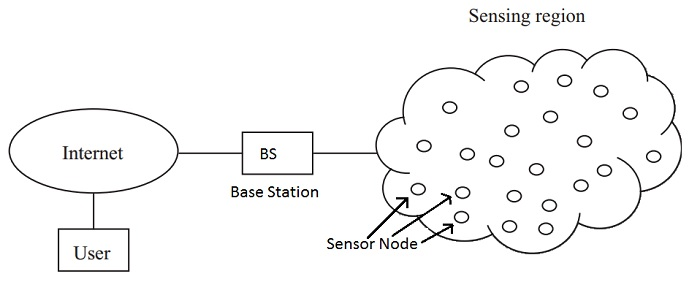
\includegraphics[scale=0.6]{wsn-arc.jpg}  
    	\caption[Arsitektur \textit{Wireless Sensor Network}]{Arsitektur \textit{Wireless Sensor Network}} 
    	\label{fig:Arsitektur Wireless Sensor Network} 
    \end{figure} 

\begin{enumerate}
    \item \textit{Flat}
    
    Pada arsitektur \textit{flat}, seluruh node sensor yang disebar memiliki tugas yang sama. Node-node tersebut melakukan \textit{sensing}, dan mengirimkan data ke \textit{base station}. Data hasil \textit{sensing} yang didapatkan oleh node sensor dapat langsung diteruskan ke \textit{base stasion} tanpa memerlukan perantara.
    
    \begin{figure}[H]
    	\centering  
    	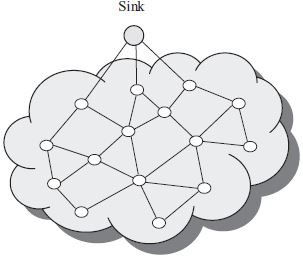
\includegraphics[scale=0.9]{flat-arch.jpg}  
    	\caption[\textit{Arsitektur \textit{Flat}}]{Arsitektur \textit{Flat}}
    	\label{fig:Aristektur Flat} 
    \end{figure}
    
    \item \textit{Hirarkikal}

    Berbeda dengan arsitektur \textit{flat} pada arsitektur \textit{hirarkikal} pengiriman hasil \textit{sensing} oleh node sensor tidak dapat secara langsung dikirimkan ke \textit{base station}. Arsitekur \textit{Hirarkikal} mengelompokan node-node yang disebar menjadi beberapa kelompok yang disebut dengan \textit{cluster}. Tiap \textit{cluster} terdiri dari sebuah \textit{ cluster head} dan \textit{cluster member}.\textit{ Cluster head} bertindak sebagai penerima data hasil sensing dari \textit{cluster member}, untuk diteruskan ke \textit{base station}.
    
    Pada arsitektur \textit{hirarkikal}, jenis komunikasi dapat dipilih berdasarkan jarak antara \textit{cluster head} ke \textit{cluster membe}r. Jenis-jenis komunikasi yang terdapat pada arsitektur hirarkikal adalah \textit{single hop} dan \textit{multi hop}. Perbedaan jenis komunikasi ini terletak pada jumlah \textit{hop} atau 'lompatan' yang dibutuhkan paket untuk mencapai tujuan.
    
    \begin{itemize}
        \item \textit{Single hop}
        
        Pada jaringan \textit{single hop}, data yang dikirimkan oleh \textit{cluster member} hanya membutuhkan satu kali lompatan (\textit{hop} tunggal) untuk mencapai \textit{cluster head}. Dengan kata lain, data yang diterima oleh \textit{cluster member} dapat langsung diterima oleh \textit{cluster head}, untuk diteruskan ke \textit{base station}.
        
        \begin{figure}[H]
        	\centering  
        	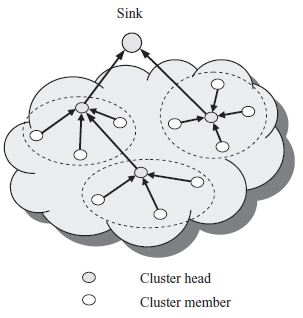
\includegraphics[scale=1]{single-hop.jpg}  
        	\caption[Arsitektur \textit{Single Hop}]{Arsitektur \textit{Single Hop}}
        	\label{fig:Arsitektur Single Hop} 
        \end{figure} 
        
        \item\textit{Multi hop}
        
        Pada jaringan \textit{multi hop}, data yang dikirimkan oleh \textit{cluster member} membutuhkan lebih dari satu kali lompatan untuk mencapai \textit{cluster head}. Data yang diterima oleh \textit{cluster head} dari \textit{cluster member}, akan diteruskan ke \textit{cluster member} lain yang memiliki jarak lebih dekat dengan \textit{cluster head}. Hal ini akan dilakukan berulang-ulang sampai paket sampai di \textit{cluster head} untuk diteruskan ke \textit{base station}.
        
        \begin{figure}[H]
        	\centering  
        	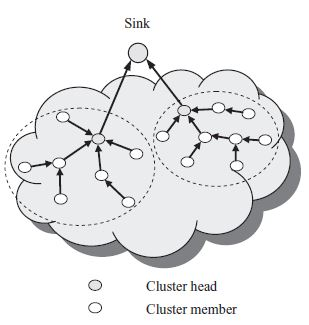
\includegraphics[scale=1]{multi-hop.JPG}  
        	\caption[Arsitektur \textit{Multi Hop}]{Arsitektur \textit{Multi Hop}}
        	\label{fig:Arsitektur Multi Hop} 
        \end{figure} 
        
    \end{itemize}
\end{enumerate}

\subsection{Topologi \textit{Wireless Sensor Network}} \label{Topologi WSN}
Topologi digunakan untuk menjelaskan hubungan antar node, dan dasar penyusunan jaringan secara geometris. Terdapat beberapa jenis topologi dalam WSN, yang tiap jenisnya memiliki fungsionalitasnya masing-masing. Pemilihan jenis topologi dipengaruhi oleh tujuan, skala jaringan, kondisi lingkungan, dan hal lainnya. Beberapa topologi jaringan pada WSN antara lain topologi \textit{bus}, topologi \textit{tree}, topologi \textit{star}, topologi \textit{ring}, topologi \textit{point-to-point}, dan topologi \textit{mesh}.
\begin{enumerate}
    \item Topologi \textit{Bus}
    
    Pada topologi bus, node-node sensor akan terhubung pada sebuah jalur. Jalur ini digunakan node-node tersebut untuk saling berkomunikasi. Komunikasi node pada topologi bus bersifat satu arah, yang mengartikan bahwa komunikasi node dilakukan secara bergantian. Komunikasi dilakuan dengan cara paket yang ingin dikirimkan oleh node pengirim akan di-\textit{broadcast} ke node sensor lain yang berada dalam jaringan. Node-node lain akan menerima paket yang dikirimkan, namun hanya sensor yang dituju yang dapat memproses hasil paket yang diterima. Topologi ini mudah udah diimplementasikan, namun untuk jaringan dengan skala yang besar, topologi ini dapat mengakibatkan kerugian dari sisi keamanan maupun \textit{bandwith}. 
    
    \begin{figure}[H]
    	\centering  
    	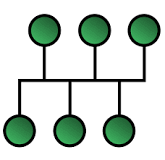
\includegraphics[scale=0.85]{bus-network.png}  
    	\caption[Topologi \textit{Bus}]{Topologi \textit{Bus}}
    	\label{fig:Topologi Bus} 
    \end{figure} 
    
    \item Topologi \textit{Star}
    
    Pada topologi \textit{star} node-node yang terhubung tidak dapat secara langsung berkomunikasi dengan node lainnya. Node-node dalam jaringan terhubung dengan \textit{main device} (\textit{central node}). Sifat \textit{main device} terbagi menjadi dua, pasif dan aktif. \textit{Main device} yang pasif hanya bertugas sebagai perantara komunikasi saja, sehingga pesan yang dikirimkan oleh node yang dikirimkan ke \textit{central node } akan diterima oleh seluruh node lain dalam jaringan. Pada \textit{main device} yang bersifat aktif bertindak sebagai pengontrol komunikasi antar node, sehingga pesan yang dikirimkan oleh node pengirim akan diteruskan oleh \textit{central node} ke node tujuan saja. Bentuk jaringan topologi \textit{star} meminimalisir adanya gangguan jika ada salah satu node yang mati. Namun, jika \textit{central node} pada jaringan ini mati atau mengalami gangguan, maka seluruh komunikasi node juga akan terhenti.
    
    \begin{figure}[H]
    	\centering  
    	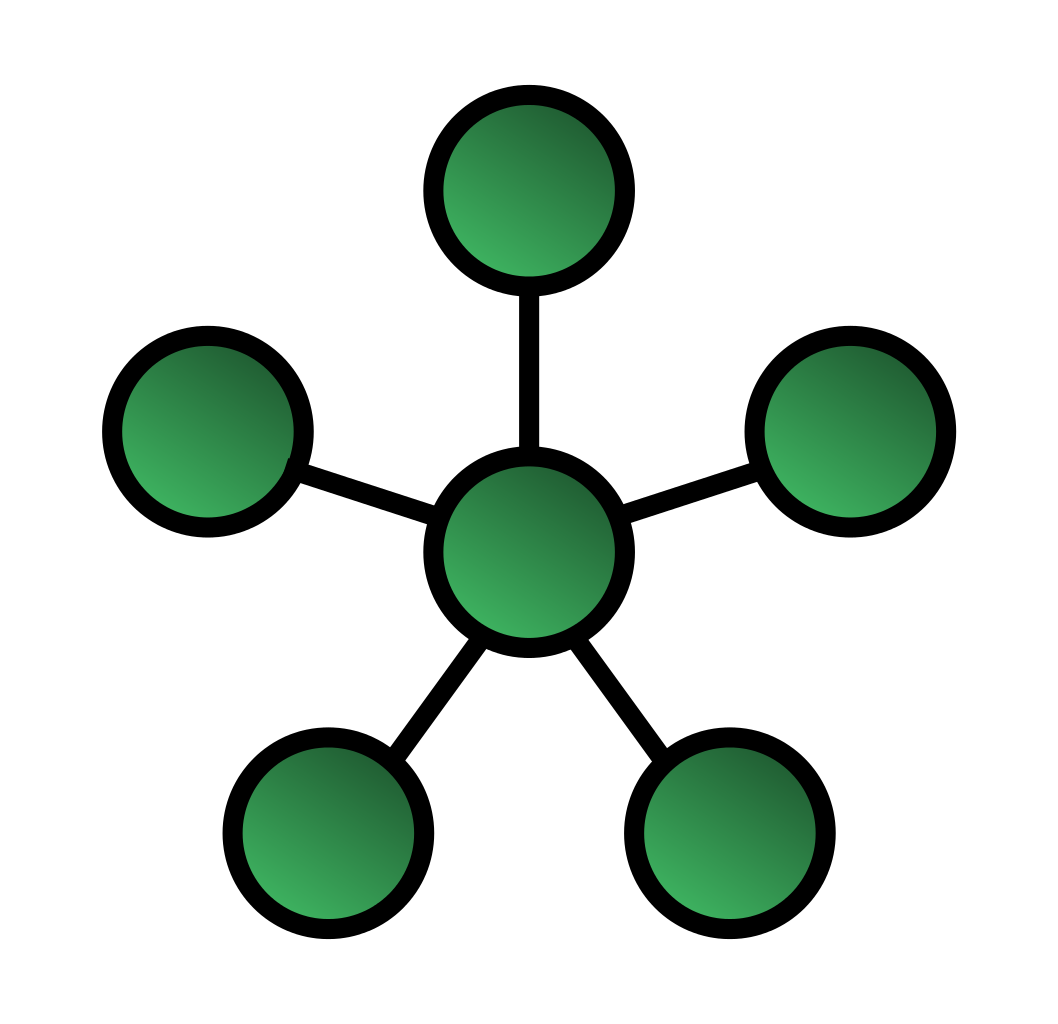
\includegraphics[scale=0.15]{star-network.png}  
    	\caption[Topologi \textit{Star}]{Topologi \textit{Star}}
    	\label{fig:Topologi Star} 
    \end{figure}
    
    \item Topologi \textit{Tree}
    
    Pada topologi \textit{tree}, rangkaian jaringan disusun secara hirarki dengan sebuah node yang berada pada level teratas yang disebut dengan \textit{root node}. Root note juga bertindak sebagai komunikasi router utama. Node-node yang berada di bawah root node disebut dengan \textit{children} atau \textit{parent}, bergantung dari kondisi node lain yang terhubung dengan node tersebut. Node yang terhubung dengan node lain yang memiliki \textit{level} lebih rendah disebut dengan \textit{parent}, sedangkan node yang tidak memiliki hubungan dengan node lain dengan \textit{level} lebih rendah disebut dengan \textit{children}. Penggunaan topologi lebih mudah untuk melakukan identifikasi dan meminimalisir kesalahan, namun hirarki pada topologi ini dapat mengakibatkan putusnya komunikasi pada \textit{children} jika salah satu \textit{parent} putus atau mati. Kelemahan lain dari topologi ini adalah sulit untuk dikonfigurasi apabila \textit{level} pada rangkaian jaringan sudah cukup besar seperti pada Gambar~\ref{fig:Jaringan Star pada Topologi Tree}.
    
    \begin{figure}[H]
    	\centering  
    	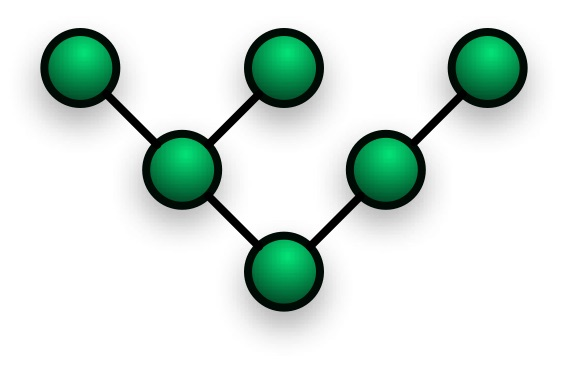
\includegraphics[scale=0.3]{tree-network-1.jpg}  
    	\caption[\textit{Topologi \textit{Tree}}]{Topologi \textit{Tree}}
    	\label{fig:Topologi Tree} 
    \end{figure}
    
    \begin{figure}[H]
    	\centering  
    	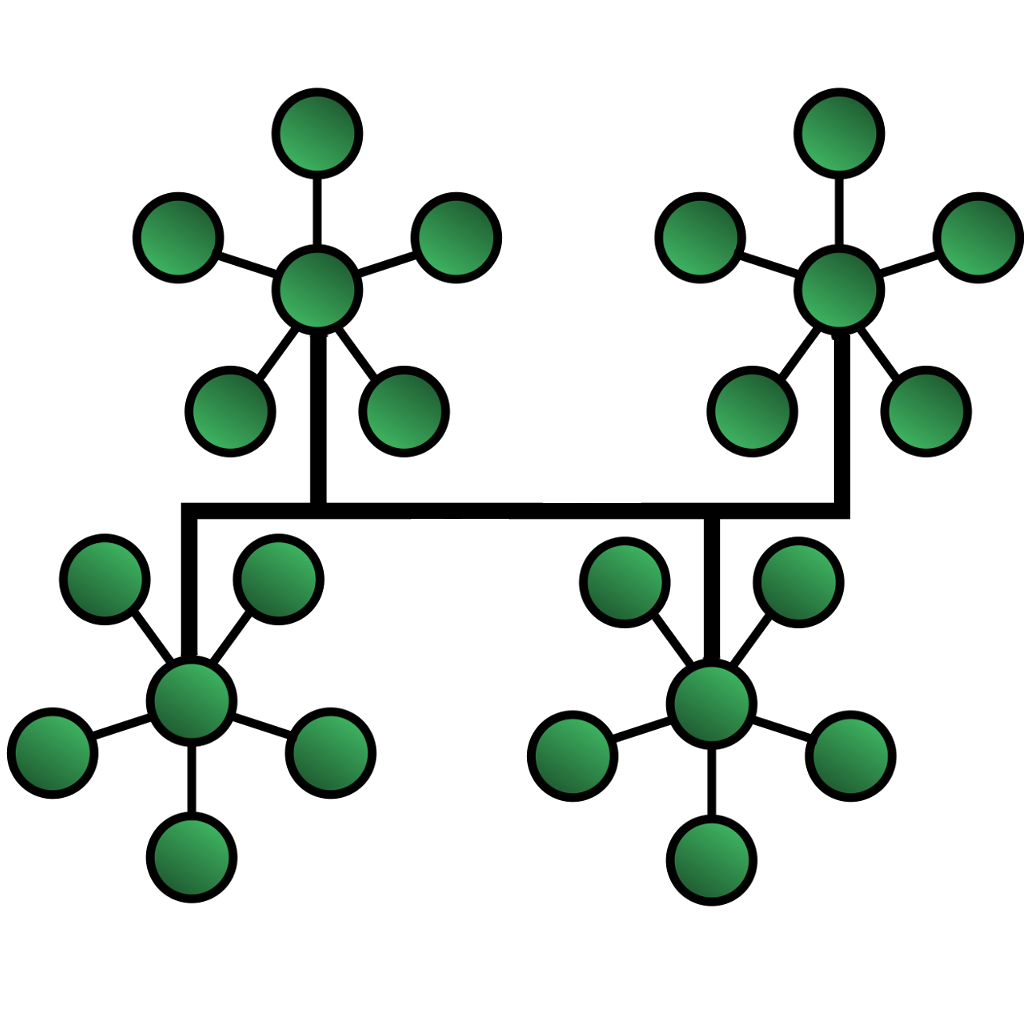
\includegraphics[scale=0.22]{tree-network-2.jpg}  
    	\caption[Jaringan \textit{Star} pada Topologi \textit{Tree}]{Jaringan \textit{Star} pada Topologi \textit{Tree}}
    	\label{fig:Jaringan Star pada Topologi Tree} 
    \end{figure}
    
    
    \item Topologi \textit{Ring}
    
    Berbeda dengan topologi \textit{star}, jaringan topologi ring tidak memiliki \textit{central node} di dalamnya. Jaringan topologi \textit{ring} berbetuk rangkaian node yang saling terhubung ke dua node lainnya (node yang paling dekat) dan membentuk lingkaran seperti cincin. Pada topologi ini, pesan node sensor pengirim akan diteruskan oleh node yang tetangganya. Proses komunikasi pengiriman pesan ini akan dilakukan terus menerus, sampai pesan yang dikirimkan oleh node pengirim diterima oleh node yang dituju. Proses komunikasi yang dilakukan pada jaringan ini mengikuti jalur melingkar (searah jarum jam ataupun sebaliknya) yang terbentuk seperti pada Gambar~\ref{fig:Topologi Ring}. Bentuk jaringan yang saling bekergantungan antara node dengan node tetangganya, dapat mengakibatkan putusnya seluruh komunikasi apabila salah satu node dalam jaringan mati.
    
    \begin{figure}[H]
    	\centering  
    	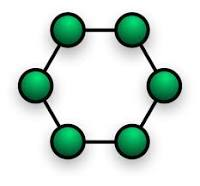
\includegraphics[scale=0.85]{ring-network.jpg}  
    	\caption[Topologi \textit{Ring}]{Topologi \textit{Ring}}
    	\label{fig:Topologi Ring} 
    \end{figure}
    
    \item Topologi \textit{Linear}
    
    Topologi \textit{linear} memiliki bentuk jaringan yang paling sederhana dibandingkan dengan topologi lainnya. Topologi ini menghubungkan node dengan node lainnya secara linear. Topologi \textit{linear} juga merupakan pengembangan dari topologi \textit{point-to-point} yang hanya membutuhkan dua buah node. Bentuk jaringan topologi linear yang sederhana membuatnya lebih mudah dikembangkan dan murah. Namun, topologi ini memiliki kekurangan yang sama dengan topologi \textit{ring}. Matinya salah satu node dalam jaringan, dapat berakibat putusnya seluruh komunikasi jaringan.
    
    \begin{figure}[H]
    	\centering  
    	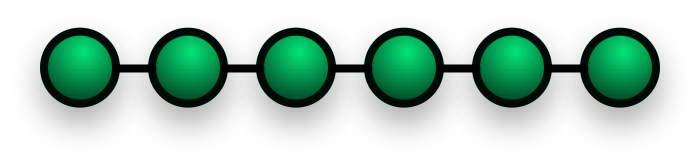
\includegraphics[scale=0.3]{line-network.png}  
    	\caption[Topologi \textit{Linear}]{Topologi \textit{Linear}}
    	\label{fig:Topologi Linear} 
    \end{figure}
    
    \item Topologi \textit{Mesh} 
    
    Terdapat dua jenis bentuk jaringan pada topologi \textit{mesh}, yaitu \textit{partially connected mesh} dan \textit{fully connected mesh}. Perbedaan kedua jaringan ini terletak pada hubungan antar node. Pada \textit{partially connected mesh}, suatu node dapat terhubung dengan node lainnya secara bebas. Pada \textit{fully connected mesh}, setiap node harus terhubung dengan seluruh node lain yang berada di dalam jaringan. Bentuk jaringan pada topologi ini memungkikan minimalnya gangguan yang terjadi apabila terdapat salah satu node mati di dalam jaringan. Namun, besarnya bentuk jaringan ini membuat sulitnya melakukan perawatan atau \textit{maintenance}.
    
    \begin{figure}[H]
    	\centering  
    	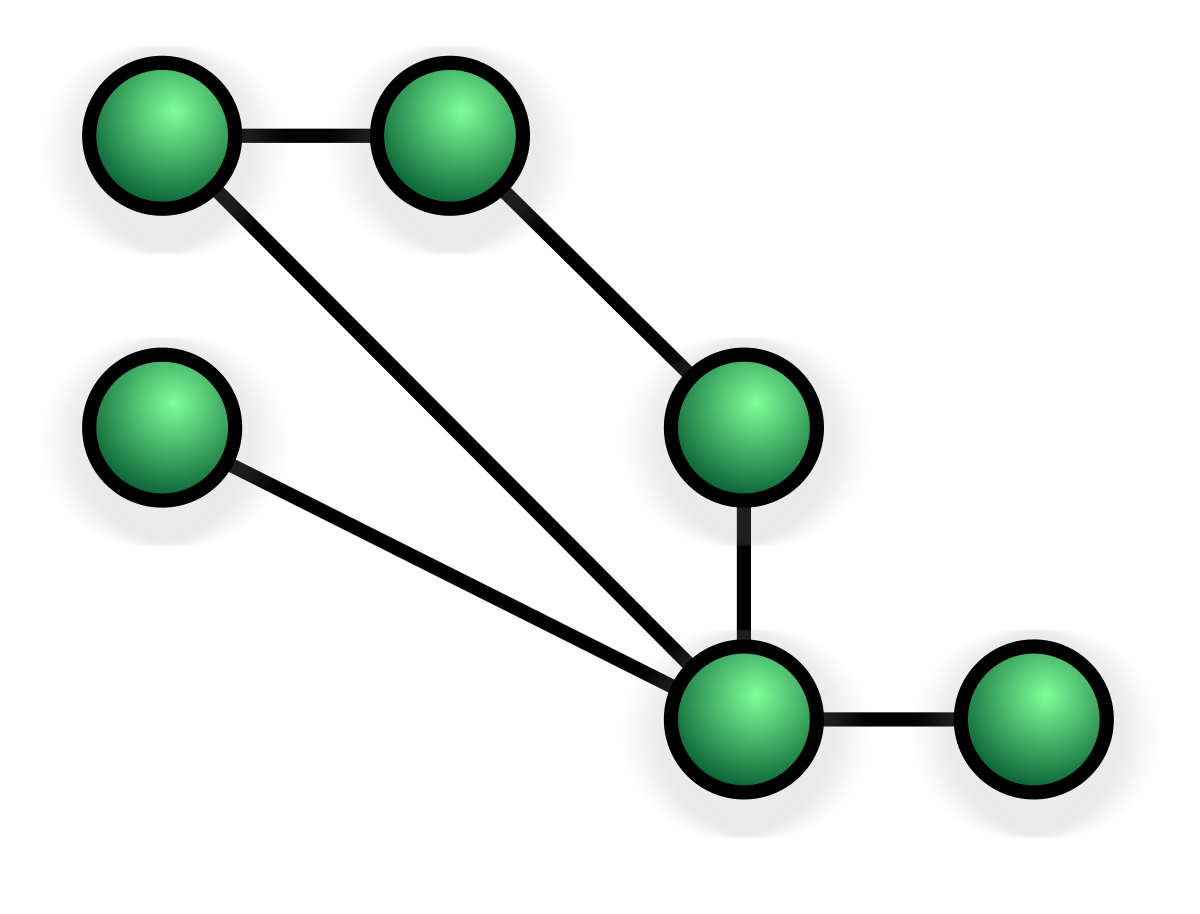
\includegraphics[scale=0.13]{mess-network-1.png}  
    	\caption[\textit{Partially connected mesh}]{\textit{Partially connected mesh}}
    	\label{fig:Partially connected mesh}
    \end{figure}
    
    \begin{figure}[H]
    	\centering  
    	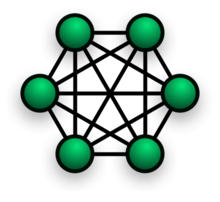
\includegraphics[scale=0.7]{full-mess-network.png}  
    	\caption[\textit{Fully connected mesh}]{\textit{Fully connected mesh}}
    	\label{fig:Fully connected mesh} 
    \end{figure}
    
\end{enumerate}

\subsection{Protokol \textit{Wireless Sensor Network}}
Protokol jaringan pada \textit{Wireless Sensor Network} biasa disebut dengan WSN \textit{protocol stack}. Protokol jaringan ini terdiri dari lima \textit{layer} atau lapisan. \textit{Layer-layer} yang menyusun protokol jaringan WSN, terdiri dari \textit{application layer, transport layer, network layer, data link layer} dan \textit{physical layer}.

\begin{itemize}
    \item \textit{Application Layer}
    
    \textit{Application Layer} merupakan lapisan yang bertindak sebagai penyedia antar muka aplikasi. Aplikasi yang dimaksud adalah aplikasi yang digunakan untuk melakukan komunikasi di dalam jaringan. Application Layer terdiri dari sejumlah protokol yang disebut dengan \textit{aplication layer protocol}. Protokol ini digunakan untuk aplikasi sensor \textit{network}.
    
    \item \textit{Transport Layer}
    
    \textit{Transport layer} memiliki tugas untuk mengirimkan data yang bersifat \textit{reliable} antar node sensor ataupun node sensor ke \textit{base station}. Cara pengiriman yang dilakukan oleh \textit{transport layer} terbagi menjadi dua jenis, yaitu \textit{upstream} dan \textit{downstream}. Perbedaan cara pengiriman ini dapat dilihat berdasarkan sumber pengirim dan penerima data. Pada \textit{upstream}, node sensor bertindak sebagai pengirim data, dan \textit{base station} bertindak sebagai penerima data. \textit{Downstream} merupakan kebalikan dari \textit{upstream}. Pada \textit{downstream}, yang bertindak sebagai pengirim data adalah \textit{base sation}, sedangkan yang bertindak sebagai penerima data adalah node sensor.\\
    Masing-masing cara pengiriman, memiliki kebutuhan \textit{reliability} yang berbeda-beda. Pada jenis pengiriman \textit{upstream}, kebutuhan \textit{reliability} tidak terlalu dibutuhkan. Hal ini disebabkan data yang dikirimkan oleh node sensor ke \textit{base station} dilakukan secara berulang-ulang, sehingga data yang tidak \textit{reliable} dapat ditoleransi. Berbeda dengan jenis pengiriman \textit{downstream}, kebutuhan \textit{reliability} sangat dibutuhkan. Pada pengiriman \textit{downstream}, jika data yang dikirimkan tidak \textit{realiable} maka aplikasi tidak dapat dijalankan. 
    
    \item \textit{Network Layer}
    
    \textit{Network Layer} merupakan lapisan ketiga dari protokol WSN. Network layer bertugas untuk menentukan jenis komunikasi antar node, \textit{single hop} atau \textit{multi hop}. \textit{Network layer} juga merupakan lapisan yang menyediakan jalur komunikasi jaringan. Data yang dikirimkan melalui lapisan ini disebut dengan paket. Paket akan dikirimkan melalui jalur yang telah disediakan dan dikendalikan oleh \textit{network layer}.
    
    \item \textit{Data Link Layer}
    
    \textit{Data Link layer} adalah lapisan yang bertindak untuk melakukan kontrol terhadap akses media yang dilakukan oleh node sensor, dan mencegah adanya paket yang bertabrakan. Proses kontrol ini juga biasa disebut dengan \textit{Medium Access Control }(MAC), sedangkan jaringan yang digunakan mencegah tabrakan antar paket disebut dengan \textit{Carrier Sense Multiple Access with Collision Avoidance}(CSMA-CA). Data link layer juga memiliki tugas untuk melakukan \textit{multiplexing} pada aliran data, membentuk \textit{data frame}, mendeteksi \textit{data frame}, \textit{medium access}, dan mendeteksi kesalahan yang mungkin terjaadi saat melakukan pengiriman data.
    
    \item \textit{Physical Layer}
    
    Physical layer merupakan lapisan yang bertindak sebagai \textit{converter} yang mengubah bit stream dari data link layer menjadi sinyal yang cocok untuk media komunikasi yang tersedia. Konversi ini dilakukan agar transmisi dapat dilakukan melalui \textit{transceiver}. \textit{Radio Frequency} (RF) digunakan untuk melakukan konfersi tersebut.  RF cukup sering digunakan pada node sensor, dikarenakan biaya yang murah, dan ukuran perangkat yang kecil.
    
    
\end{itemize}

Selain lima \textit{layer} yang disebutkan, terdapat tiga \textit{layer} lain yang terletak di bidang lintas lapisan yang terdiri dari \textit{task management plane, mobility management plane}, dan \textit{power management plane}.

\begin{itemize}
    \item \textit{Power management plane}
    
    \textit{Power management plane} bertindak sebagai pengontrol penggunaan sumber daya atau energi untuk setiap node sensor. Pengaturan sumber daya oleh power management plane dilakukan pada saat node sensor melakukan \textit{sensing}, \textit{processing}, ataupun saat \textit{transmission} dan \textit{reception} (mengirim dan menerima data). 
    
    \item \textit{Connection management plane}
    
    \textit{Connection management plane} berfungsi untuk melakukan konfigurasi terhadap segala sesuatu yang berkaitan dengan koneksi antar node sensor. Konfigurasi atau rekonfigurasi biasa dilakukan saat terjadi perubahan topologi pada wireless sensor network. 
    
    \item \textit{Task management plane}
    
   \textit{Task management plane} memiliki tugas untuk melakukan pembagian atau distribusi tugas (task) untuk setiap node sensor. Pembagian tugas ini dilakukan agar penggunaan energi dapat dioptimalkan dan lebih efisien.
    
\end{itemize}

    \begin{figure}[H]
    	\centering  
    	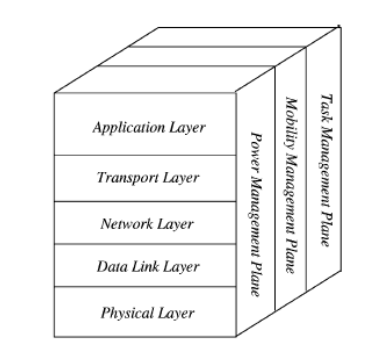
\includegraphics[scale=0.75]{protokol-jaringan.png}  
    	\caption[Protokol Jaringan]{Protokol Jaringan}
    	\label{fig:Protokol Jaringan} 
    \end{figure}

% Berikut adalah contoh pembuatan tabel. 
% Penempatan tabel dan gambar secara umum diatur secara otomatis oleh \LaTeX{}, perhatikan contoh di file bab2.tex untuk melihat bagaimana cara memaksa tabel ditempatkan sesuai keinginan kita.

% Perhatikan bawa berbeda dengan penempatan judul gambar gambar, keterangan tabel harus diletakkan di atas tabel!!
% Lihat Tabel~\ref{tab:contoh1} berikut ini:

% \begin{table}[H] %atau h saja untuk "kira kira di sini"
% 	\centering 
% 	\caption{Tabel contoh}
% 	\label{tab:contoh1}
% 	\begin{tabular}{cccc}
% 		\toprule
% 		& $v_{start}$ & $\mathcal{S}_{1}$ & $v_{end}$\\

% 		\midrule
% 		$\tau_{1}$ & 1 & 12& 20\\
% 		$\tau_{2}$ & 1 &  & 20\\
% 		$\tau_{3}$ & 1 & 9 & 20\\
% 		$\tau_{4}$ & 1 &  & 20\\

% 		\bottomrule
		
% 	\end{tabular} 
% \end{table}
% Tabel~\ref{tab:cthwarna1} dan Tabel~\ref{tab:cthwarna2} berikut ini adalah tabel dengan sel yang berwarna dan ada dua tabel yang bersebelahan. 
% \begin{table}[H]
% 	\begin{minipage}[c]{0.49\linewidth}
% 		\centering
% 		\caption{Tabel bewarna(1)}
% 		\label{tab:cthwarna1}
% 		\begin{tabular}{ccccc}
% 			\toprule
% 			 & $v_{start}$ & $\mathcal{S}_{2}$ & $\mathcal{S}_{1}$ & $v_{end}$\\
			
% 			\midrule
% 			$\tau_{1}$ & 1 & 5 \cellcolor{green}& 12& 20\\
% 			$\tau_{2}$ & 1 & 8 \cellcolor{green}& & 20\\
% 			$\tau_{3}$ & 1 & 2/8/17 \cellcolor{green}& 9 & 20\\
% 			$\tau_{4}$ & 1 & \cellcolor{red}& & 20\\
			
% 			\bottomrule

% 		\end{tabular}
% 	\end{minipage}
% 	\begin{minipage}[c]{0.49\linewidth}
		
% 		\centering 
% 		\caption{Tabel bewarna(2)}
% 		\label{tab:cthwarna2}
% 		\begin{tabular}{ccccc}
% 			\toprule
% 			 & $v_{start}$ & $\mathcal{S}_{1}$ & $\mathcal{S}_{2}$ & $v_{end}$\\
			
% 			\midrule
% 			$\tau_{1}$ & 1 & 12& 5 \cellcolor{red} &20\\
% 			$\tau_{2}$ & 1 &  &  8 \cellcolor{green} &20\\
% 			$\tau_{3}$ & 1 & 9 & 2/8/17 \cellcolor{green} &20\\
% 			$\tau_{4}$ & 1 &   & \cellcolor{red} &20\\
			
% 			\bottomrule
		
% 		\end{tabular}
% 	\end{minipage}
% \end{table}
\section{Zigbee}
Zigbee merupakan standar spesifikasi untuk jaringan protokol yang menggunakan radio digital. Protokol zigbee berbasiskan pada standar IEEE 802.15.4-2003 untuk jaringan nirkabel tingkat rendah. Kebutuhan konsumsi daya yang rendah untuk zigbee beroperasi, menjadi solusi untuk perangkat yang memiliki persediaan daya terbatas. Oleh karena itu, zigbee biasa digunakan dalam perangkat yang menggunakan baterai. Zigbee juga biasa digunakan untuk aplikasi pengontrolan atau pemantauan yang bersifat nirkabel, seperti  alarm peringatan kebakaran (asap) ataupun diteksi penyusup. Zigbee juga merupakan spesifikasi standar yang digunakan dalam jaringan nirkabel \textit{mesh}.

Pada umumnya, chip yang terpasang pada zigbee telah terintegrasi dengan mikrokontroler dan tidak membutuhkan \textit{memory} yang besar. Namun, zigbee hanya dapat mengirimkan komunikasi dengan latensi yang rendah (\textit{low-latency communication}). Rendahnya latensi komunikasi yang dimiliki oleh zigbee menyebabkan kurang tepatnya penggunaan zigbee untuk perangkat yang memerlukan kecepatan transfer data yang tinggi.

\subsection{Jenis-jenis perangkat zigbee}
Terdapat tiga jenis perangkat zigbee antara lain:
\begin{itemize}
    \item ZigBee Coordinator (ZC)
    
    Zigbee Coordinator merupakan perangkat yang digunakan sebagai repositori informasi jaringan maupun keamanan. Zigbee Coordinator juga merupakan perangkat pertama yang beroperasi ketika jaringan diaktifkan. Hal ini dikarenakan Zigbee Coordinator membentuk dasar dari jaringan dan menghubungkan jaringan-jaringan lainnya.  
        
    \item ZigBee Router (ZR)
    
    Zigbee Router merupakan perangkat yang bertindak sebagai perantara dalam pengiriman atau penyampaian data. Selain berfungsi untuk meneruskan data antar perangkat, Zigbee router juga bertindak dalam menjalankan fungsi aplikasi. 
    
    \\~\\
    
    \item ZigBee End Device (ZED)
    
    Zigbee End Device adalah perangkat yang berperan sebagai parent node. Hal tersebut menyebabkan Zigbee End Device tidak dapat mengirim ulang ataupun meneruskan data dari perangkat lain. Peran zigbee sebagai parent node terjadi pada koordinator maupun router.
\end{itemize}


 
\section{Arduino} 
Arduino adalah perangkat keras pengendali mikrokontroler yang bersifat \textit{open-source} untuk membangun perangkat digital. Arduino dirancang untuk menjadi alternatif bagi pelajar dalam membangun perangkat digital yang dapat berkomunikasi dengan lingkungan, dengan harga yang lebih murah. Mikrokontroler arduino dapat diprogram menggunakan bahasa pemrograman C. Kompiler dan Integrated Development Enviroment (IDE) untuk proyek yang menggunakan arduino-pun juga sudah banyak tersedia. 

\subsection{Jenis-jenis arduino}
Arduino memiliki banyak jenis mikrokontroler dengan spesifikasi yang berbeda-beda. Jumlah pin \textit{input/output} ,jenis chip, dan modul yang tersedia bergantung pada tipe arduino yang digunakan.

\begin{enumerate}
    \item Arduino Uno
    
    \begin{figure}[H]
    	\centering  
    	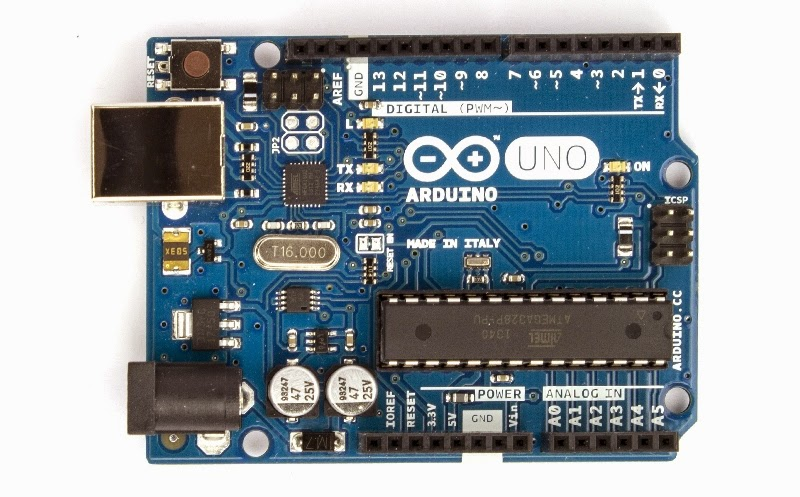
\includegraphics[scale=0.25]{arduino-uno.jpg}  
    	\caption[Arduino Uno]{Arduino Uno} 
    	\label{fig:Arduino Uno} 
    \end{figure} 

    Arduino uno merupakan mikrokontroler yang paling populer dan paling sering digunakan. Referensi yang membahas mengenai arduino uno juga sudah cukup banyak, sehingga mudah untuk dipelajari untuk para pemula. Arduino uno menggunakan ATMEGA328P sebagai mikrokontrolernya, dan dilengkapi dengan 14 pin input/output digital dan 6 pin input analog. Untuk pemrograman, arduino uno menggunakan koneksi USB type B. Arduino Uno R3 merupakan versi terakhir dari arduino uno sampai saat ini.
    
    \item Arduino Due
    
    \begin{figure}[H]
    	\centering  
    	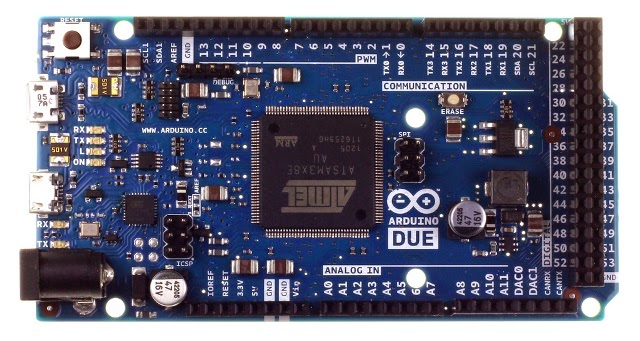
\includegraphics[scale=0.25]{arduino-due.jpg}  
    	\caption[Arduino Due]{Arduino Due} 
    	\label{fig:Arduino Due} 
    \end{figure} 
    
    Arduino Due menggunakan mikrokontroler yang lebih tinggi dibandingkan arduino uno, yaitu 32bit ARM Cortex CPU. Mikrokontroler yang digunakan pada arduino due memungkinkan pengguna untuk tetap menggunakan bahasa pemrograman yang \textit{compatible}. Node ini memiliki 54 input/output pin digital, 12 pin input analog,dan 84MHz clock. Arduino due menggunakan micro USB untuk pemrograman.
    
    \item Arduino Mega
    
    \begin{figure}[H]
    	\centering  
    	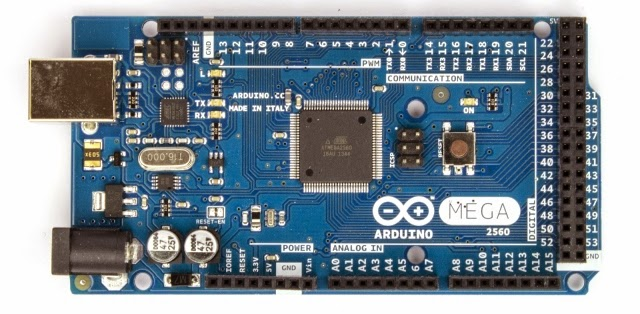
\includegraphics[scale=0.25]{arduino-mega.jpg}  
    	\caption[Arduino Mega]{Arduino Mega} 
    	\label{fig:Arduino Mega} 
    \end{figure} 
    
    Arduino Mega merupakan pengembangan dari arduino uno. Keduanya menggunakan USB type B untuk pemrogramannya. Namun, arduino mega menggunakan chip yang lebih tinggi yaitu ATMEGA2560. Penggunaan chip ATMEGA2560, memungkinkan penyimpanan ukuran program yang lebih besar. Arduino mega juga memiliki ukuran papan yang lebih besar dibandingkan papan lainnya. Hal ini dikarenakan jumlah pin input/output dan pin input analognya yang lebih banyak dibandingkan arduino uno.
    
    \item Arduino Leonardo
    
    \begin{figure}[H]
    	\centering  
    	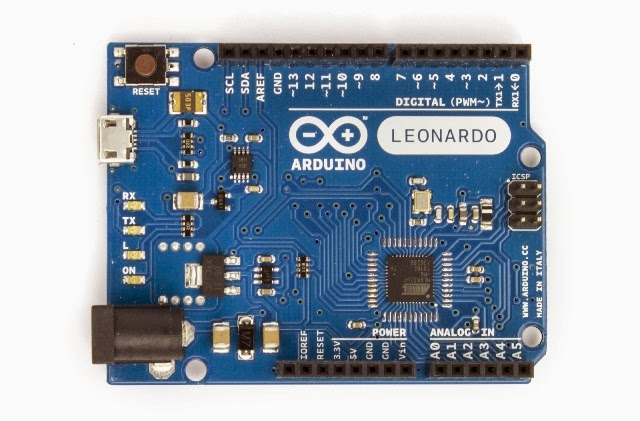
\includegraphics[scale=0.25]{arduino-leonardo.jpg}  
    	\caption[Arduino Leonardo]{Arduino Leonardo} 
    	\label{fig:Arduino Leonardo} 
    \end{figure} 
    
    Arduino Leonardo memiliki kemiripan yang hampir identik dengan arduino uno, jumlah pin input/output dan pin input analognya-pun sama dengan arduino uno. Hanya saja, Micro USB digunakan untuk pemrograman pada arduino leonardo, berbeda dengan arduino uno yang menggunakan USB type B untuk basis pemrogramannya.
    
    \item Arduino Fio
    
    \begin{figure}[H]
    	\centering  
    	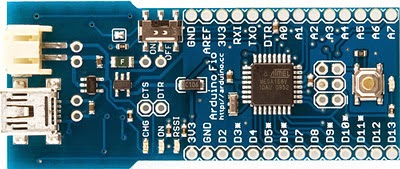
\includegraphics[scale=0.35]{arduino-fio.jpg}  
    	\caption[Arduino Fio]{Arduino Fio} 
    	\label{fig:Arduino Fio} 
    \end{figure} 
    
    Arduinio Fio menggunakan socket berbeda dengan jenis arduino lainnya. Socket yang digunakan pada arduino fio adalah XBee. Socket XBee memungkinkan arduino fio untuk digunakan dalam proyek yang mengharuskan penggunaan nirkabel. Dengan menggunakan arduino fio, pengguna dapat mengirimkan data secara \textit{wireless}.
    
    \item Arduino Nano
    
    \begin{figure}[H]
    	\centering  
    	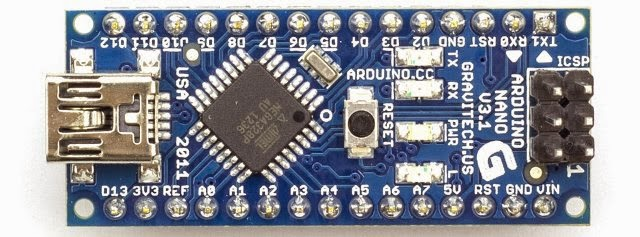
\includegraphics[scale=0.25]{arduino-nano.jpg}  
    	\caption[Arduino Nano]{Arduino Nano} 
    	\label{fig:Arduino Nano} 
    \end{figure} 
    
    Arduino nano adalah mikrokontroler dengan papan berukuran kecil. Chip yang digunakan pada arduino nano adalah ATmega328P. Untuk pemrograman, arduino nano dilengkapi dengan FTDI dengan Micro USB. Jumlah pin input analog yang dimiliki android nano lebih banyak dibandingkan dengan android uno (8 Pin). Android nano memiliki dua versi yang berbeda pada chip yang digunakannya, ATMEGA168 atau ATMEGA328.
    
    \item Arduino Mini
    
    \begin{figure}[H]
    	\centering  
    	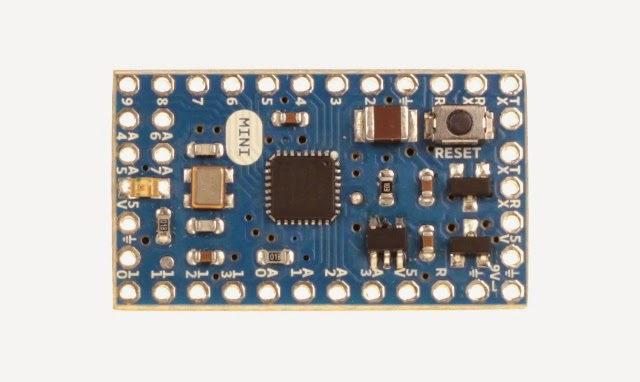
\includegraphics[scale=0.30]{arduino-mini.jpg}  
    	\caption[Arduino Mini]{Arduino Mini} 
    	\label{fig:Arduino Mini} 
    \end{figure} 
    
    Ukuran papan arduino mini yang kecil membuatnya sedikit lebih rumit untuk dihubungkan, dibandingkan denan papan arduino lainnya. Namun, ukurannya yang kecil memungkinkan arduino mini untuk digunakan pada tempat sempit yang memerlukan node sensor berukuran kecil.
    
    \item Arduino Micro
    
    \begin{figure}[H]
    	\centering  
    	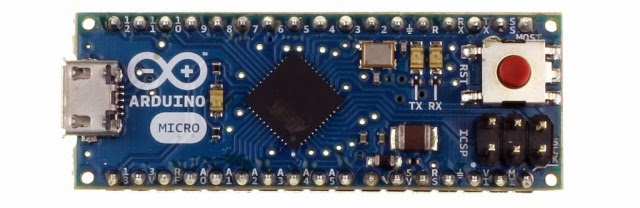
\includegraphics[scale=0.35]{arduino-micro.jpg}  
    	\caption[Arduino Micro]{Arduino Micro} 
    	\label{fig:Arduino Micro} 
    \end{figure} 
    
    Arduino micro merupakan perangkat keras kecil seperti arduino nano dan arduino mini. Namun arduino micro memiliki kelebihan dibanding perangkat arduino berukuran kecil lainnya. Mudahnya dalam mengintegrasikan arduino micro dengan benda sehari-hari menjadikannya lebih interaktif dibandingkan jenis arduino lainnya.
    
    \item Arduino Ethernet
    
    \begin{figure}[H]
    	\centering  
    	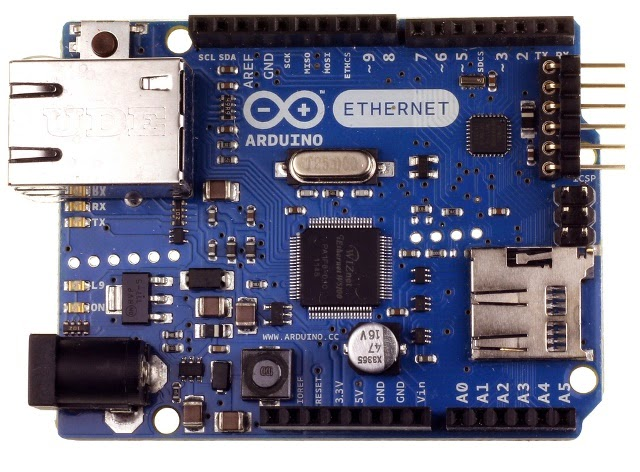
\includegraphics[scale=0.25]{arduino-ethernet.jpg} 
    	\caption[Arduino Ethernet]{Arduino Ethernet} 
    	\label{fig:Arduino Ethernet} 
    \end{figure} 
    
    Seperti namanya arduino ethernet telah dilengkapi dengan fasilitas ethernet. Dengan fitur tersebut, arduino ethernet dapat melakukan komunikasi melalui jaringan LAN pada komputer. Arduino ethernet juga dilengkapi dengan fitur \textit{reset} otomatis, yang memungkinkan pengguna untuk mengunggah  data tanpa harus menekan tombol reset.
    
    \item Arduino Esplora
    
    \begin{figure}[H]
    	\centering  
    	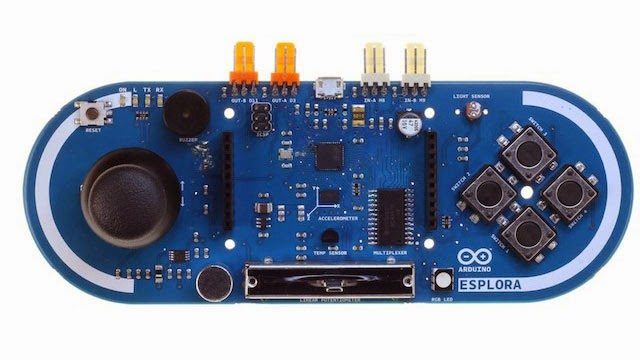
\includegraphics[scale=0.25]{arduino-esplora.jpg}  
    	\caption[Arduino Esplora]{Arduino Esplora} 
    	\label{fig:Arduino Esplora} 
    \end{figure} 
    
    Seperti arduino leonardo, arduino esplora menggunakan chip ATMEGA32U4. Namun, arduino esplora menyediakan sejumlah sensor yang telah terintegrasi dan siap untuk digunakan. Arduino esplora juga telah dilengkapi dengan \textit{joystick}, dan tombol interaksi yang terhubung dengan papan.
\end{enumerate}

\subsection{Jenis-jenis sensor \textit{sensing} arduino}
Pada setiap node yang disebar di area persawahan yang akan dilakukan pengukuran, terpasang sensor yang dapat melakukan \textit{sensing} terhadap lingkungan. Untuk pengukuran yang berkaitan dengan kondisi tanah sawah, sensor \textit{sensing} yang digunakan harus dapat mengukur variabel yang mempengaruhi kondisi tanah sawah. Sensor yang dapat mengukur faktor-faktor yang mempengaruhi kondisi tanah sawah antara lain, sensor pengukur kadar keasaman tanah (pH), sensor pengukur  kelembaban tanah, sensor pengukur suhu temperatur tanah, sensor pengukur suhu dan kelemebaban udara, dan \textit{Wireless Data Transceiver}.

\begin{enumerate}
    \item Sensor pengukur kadar keasaman tanah (pH)
    
    Rangkaian ini terdiri dari komponen sensor keasaman yang digunakan untuk melakukan pengukuran pH yang berada di tanah. Pengukuran dilakukan untuk mengetahui kandungan yang berada dalam tanah seperti Nitrogen (N), Potassium/kalium (K), dan Pospor (P) yang sangat berpengaruh terhadap tanaman padi untuk tumbuh dan menghasilkan kualitas yang baik. Contoh sensor pengukur kadar keasaman tanah ini dapat dilihat pada Gambar~\ref{fig:Sensor pengukur kadar keasaman tanah (pH)}
    
    \begin{figure}[H]
    	\centering  
    	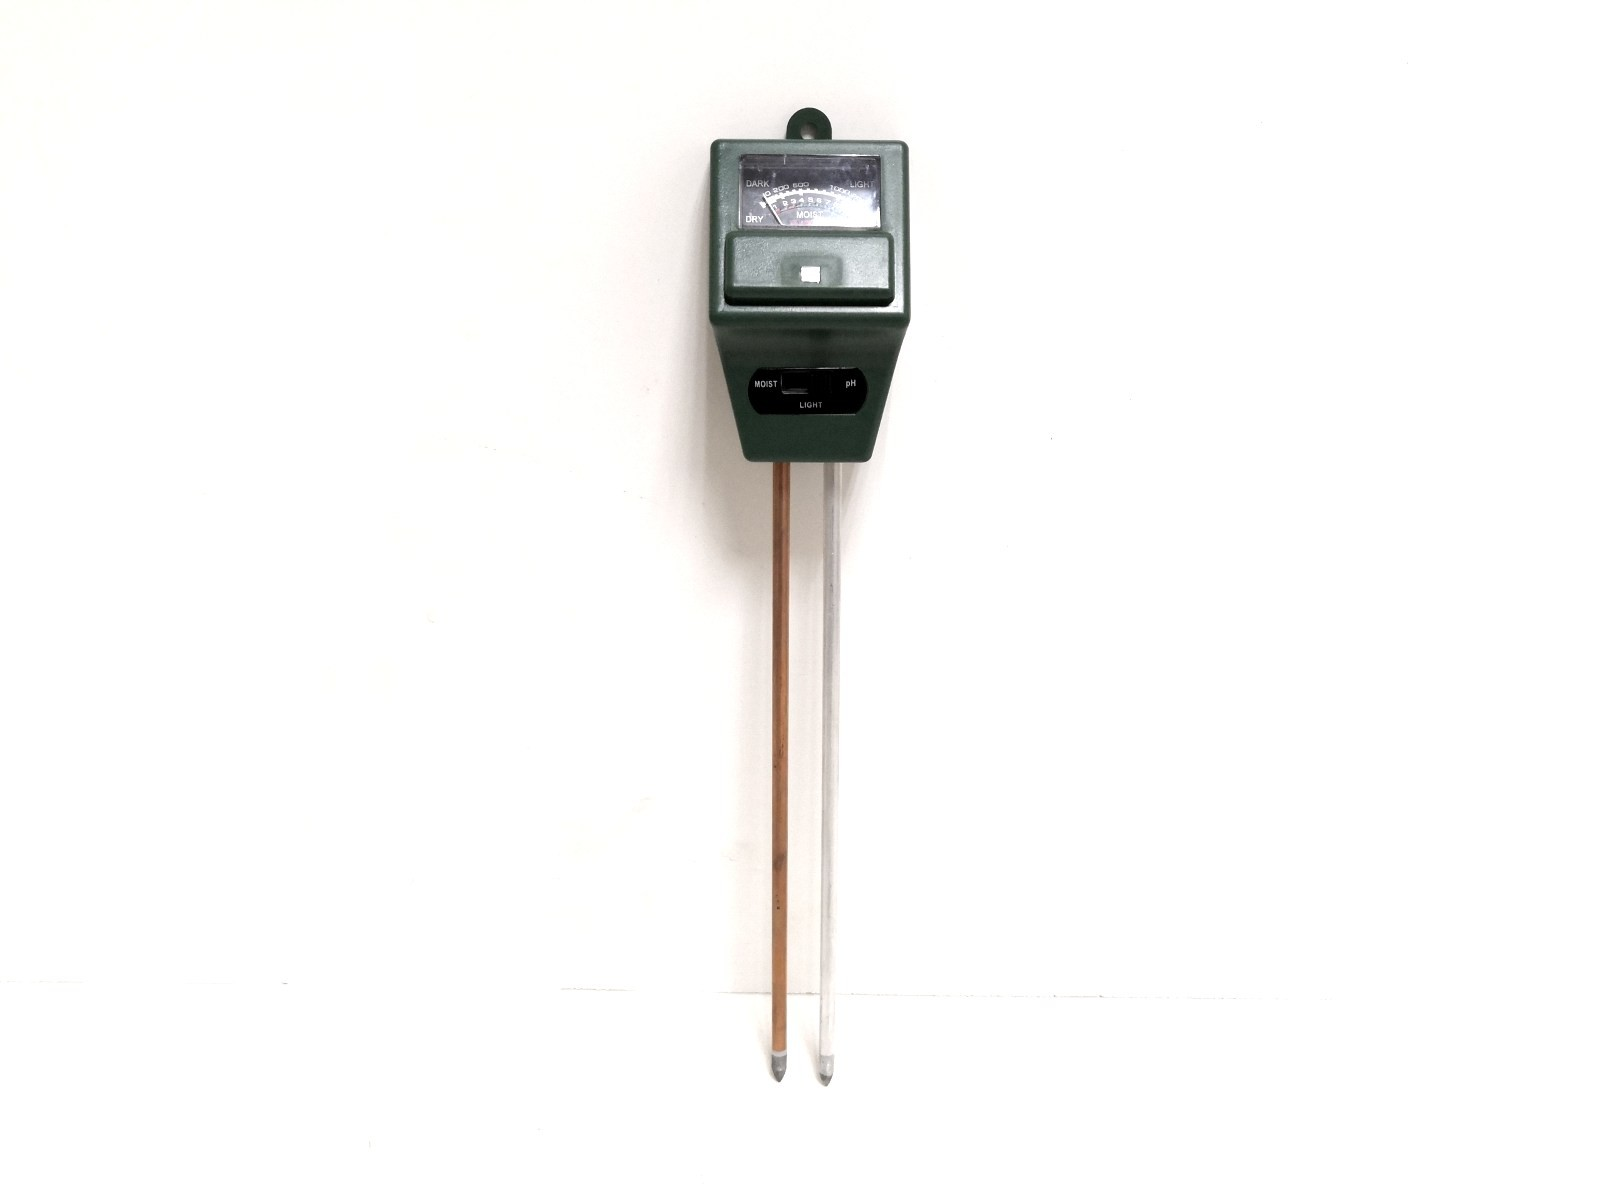
\includegraphics[scale=0.23]{ph_Meter.jpg}  
    	\caption[Sensor pengukur kadar keasaman tanah (pH)]{Sensor pengukur kadar keasaman tanah (pH)} 
    	\label{fig:Sensor pengukur kadar keasaman tanah (pH)} 
    \end{figure}
    
    \item Sensor pengukur tingkat kelembaban tanah
    
    Untuk mengetahui kadar air yang berada di dalam tanah maka diperlukan sensor kelembapan yang berfungsi untuk mendapatkan tingkat kelembapan tanah berdasarkan arus listrik yang dihantarkan. Semakin banyak kadar air dalam tanah mengindikasikan semakin lembab tanah tersebut, dan semakin tinggi tingkat kelembaban tanah maka arus listrik yang dihantarkan akan semakin tinggi (resistansi tinggi). Jika tanah memiliki kadar air yang rendah (tanah kering) maka arus listrik yang dihantarkan akan rendah (lebih banyak perlawanan). Contoh sensor pengukur tingkat kelembaban ini dapat dilihat pada Gambar~\ref{fig:Sensor pengukur tingkat kelembaban tanah}
    
    \begin{figure}[H]
    	\centering  
    	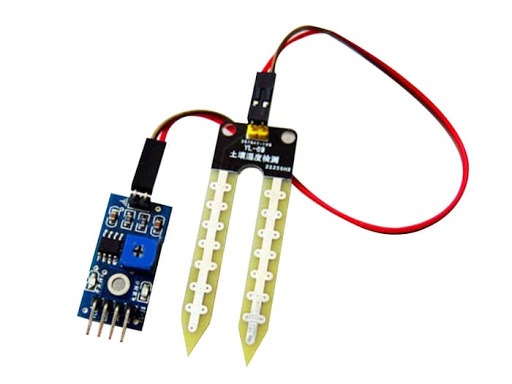
\includegraphics[scale=0.35]{sensor-kelembaban.jpg}  
    	\caption[Sensor pengukur tingkat kelembaban tanah]{Sensor pengukur tingkat kelembaban tanah} 
    	\label{fig:Sensor pengukur tingkat kelembaban tanah} 
    \end{figure} 
    
    \item Sensor pengukur suhu temperatur tanah

     Sensor suhu diperlukan untuk memantau temperature kondisi tanah sawah yang diteliti untuk mengetahui suhu telah mencapai temperature yang tepat.
     Contoh sensor pengukur suhu temperatur tanah dapat dilihat pada Gambar~\ref{fig:Sensor pengukur suhu temperatur tanah}
     
     \begin{figure}[H]
    	\centering  
    	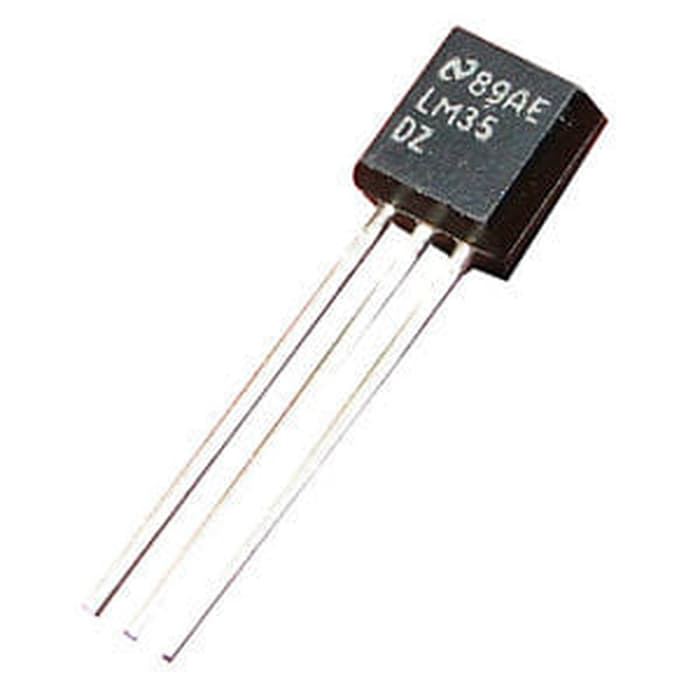
\includegraphics[scale=0.45]{sensor-suhu-tanah.jpg}  
    	\caption[Sensor pengukur suhu temperatur tanah]{Sensor pengukur suhu temperatur tanah} 
    	\label{fig:Sensor pengukur suhu temperatur tanah} 
    \end{figure}
    
    \item Sensor pengukur suhu dan kelembaban udara 

     Sensor suhu dan kelembaban udara diperlukan untuk memantau suhu dan kelembaban suatu daerah, dan mengetahui suhu udara dan tingkat kelembaban udara daerah yang diteliti telah mencapai temperature yang tepat.
     Contoh sensor pengukur suhu dan kelembaban udara dapat dilihat pada Gambar~\ref{fig:Sensor pengukur suhu kelembaban udara}
     
     \begin{figure}[H]
    	\centering  
    	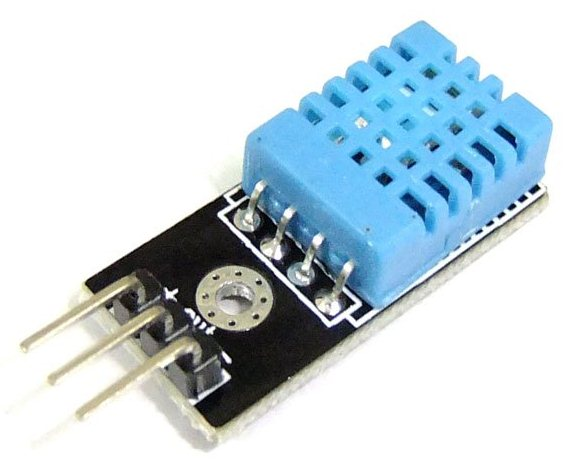
\includegraphics[scale=0.37]{sensor_suhu.jpg}  
    	\caption[Sensor pengukur suhu kelembaban udara]{Sensor pengukur suhu kelembaban udara} 
    	\label{fig:Sensor pengukur suhu kelembaban udara} 
    \end{figure}
     
     \item WDT (\textit{Wireless Data Transceiver})
     
     WDT atau \textit{Wireless Data Transceiver} digunakan untuk mengirimkan dan menerima data, tanpa memerlukan kabel sebagai perantara pengiriman. WDT juga berfungsi sebagai alat komunikasi antar node sensor. Contoh Wireless Data Transceiver dapat dilihat pada Gambar~\ref{fig:Wireless Data Transceiver}
     
     \begin{figure}[H]
    	\centering  
    	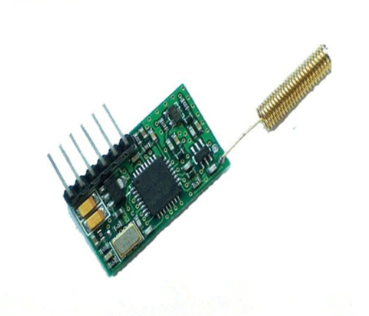
\includegraphics[scale=0.6]{wdt.png}  
    	\caption[\textit{Wireless Data Transceiver}]{\textit{Wireless Data Transceiver}} 
    	\label{fig:Wireless Data Transceiver} 
    \end{figure}
\end{enumerate}



\subsection{Pemrograman Arduino} \label{Pemrograman Arduino}
Arduino menggunakan bahasa pemrograman mandiri (bahasa pemrograman arduino) yang digunakan pada AVR. Bahasa pemrograman arduino, memiliki banyak kemiripan dengan bahasa pemrograman C. Kemiripan kedua bahasa ini dapat terlihat dari fungsi, syntax, variabel, operator matematika, operator pembanding, dan struktur pengaturan yang tersedia. Bahasa pemrograman Arduino juga sering dianggap sebagai bahasa \textit{processing}\footnote{\url{https://kelasrobot.com/belajar-pemrograman-dasar-arduino/}}.

\begin{itemize}
    \item Fungsi
    
    Program yang terdapat di arduino juga biasa disebut dengan \textit{sketch}. Terdapat dua buah fungsi yang harus ada pada setiap \textit{sketch}, yaitu fungsi setup dan fungsi loop.
    
        \begin{itemize}
            \item Void setup
            \label{void setup}
            
            Void setup merupakan fungsi pertama yang akan dieksekusi dalam pemrograman arduino sebelum fungsi atau kode lainnya. Fungsi void setup memiliki \textit{task} untuk menentukan kegunaan dari sebuah pin. Selain itu fungsi ini juga dapat digunakan untuk memulai komunikasi antara arduino dengan komputer.
            
            
            \item Void loop
            
            Semua kode yang berada di dalam fungsi ini akan dibaca setelah fungsi void setup dieksekusi, dan akan terus menerus dijalankan sampai daya yang terhubung pada perangkat dilepaskan. Fungsi ini berisikan kode-kode perintah untuk pin \textit{input} dan \textit{output} pada arduino.
            
        \end{itemize}
        
        \begin{figure}[H]
        	\centering  
        	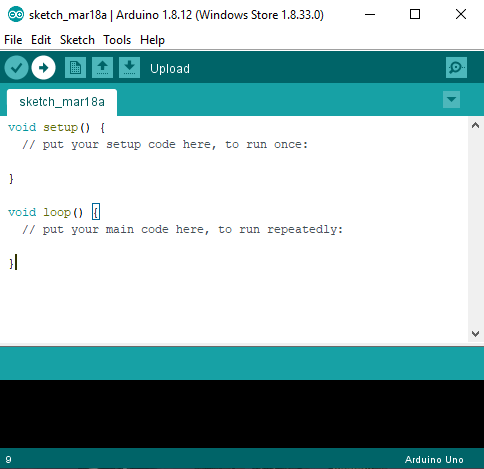
\includegraphics[scale=0.9]{setup_loop.png}  
        	\caption[Fungsi setup dan loop pada Arduino]{Fungsi setup dan loop pada Arduino} 
        	\label{fig:Fungsi setup dan loop pada Arduino} 
        \end{figure}
    
    \item Struktur pengaturan
    
    Didalam struktur pengaturan bahasa pemrograman arduino, terdapat struktur-struktur yang umum terdapat pada bahasa pemrograman lainnya. Beberapa contoh struktur pengaturan di dalam bahasa pemrograman arduino adalah \textit{loop} menggunakan \textit{for} untuk melakukan pengulangan dan penggunaan \textit{if-else} untuk pengolahan kode program dengan kondisi bercabang (\textit{branching}).
    
    \item Digital
    
    Kode digital digunakan untuk pemrograman yang menggunakan pin digital pada arduino. Kode program yang berkaitan dengan nilai digital adalah pinMode yang digunakan untuk melakukan pengaturan input-output mode pin, digitalRead yang digunakan untuk membaca nilai sensor yang terdapat pada pin, dan digitalWrite untuk melakukan pengaturan pada pin output. 
    
    \item Analog
    
    Tidak hanya mengelola hasil dalam format digital, arduino juga dapat menggunakan fungsi analognya pada pin digital arduino. Sama seperti digital fungsi \textit{read} dan \textit{write} juga dapat diolah dalam format analog.
    
    \item \textit{Blink Test}
    
    Salah satu contoh pemrograman pada Arduino yang cukup sederhana adalah mengedipkan LED \textit{on-board} pada papan Arduino, atau biasa disebut dengan \textit{blink test}. Untuk melakukan \textit{blink test}, pengguna harus memastikan jenis board yang dipilih pada IDE Arduino telah sesuai dengan perangkat keras yang digunakan (yang terhubung dengan komputer). Setelah IDE Arduino dan perangkat keras telah sesuai dan terhubung, maka pemrograman dapat dilakukan seperti Gambar~\ref{fig:Blink Test On-Board}. Setelah kode program selesai ditulis, pengguna dapat menverifikasi program dengan cara menekan tombol dengan ikon check diatas kiri IDE Arduino. Setelah kode program terverifikasi, pengguna dapat mengupload kode program tersebut ke papan arduino, dengan cara menekan tombol upload yang berada disamping tombol verifikasi. Jika upload sukses dilakukan maka IDE akan memberikan informasi "Done uploading", dan papan arduino yang terhubung akan melakukan kode perintah yang diupload. Untuk kode program pada Gambar~\ref{fig:Blink Test On-Board}, papan akan mengedipkan led on-board setiap 3 detik dengan lama lampu menyala selama 2 detik. 
    
    Blink test juga dapat digunakan untuk menguji pin yang terdapat pada papan, berfungsi dengan baik atau tidak. Blink test untuk menguji fungsional pin dapat dilakukan dengan cara memasang led eksternal pada pin yang tersedia pada papan arduino, dan menjalankan program seperti pada Gambar~\ref{fig:Blink Test Pin}.
    
        \begin{figure}[H]
        	\centering  
    	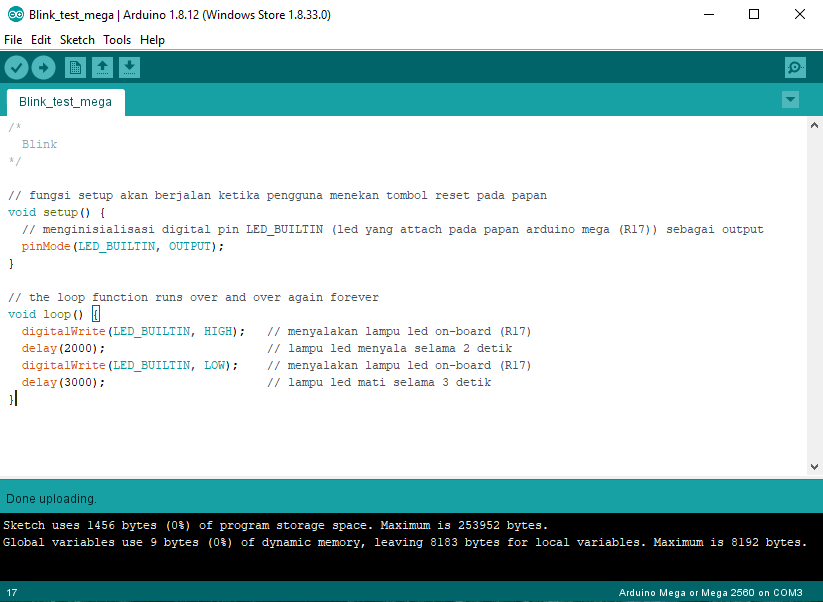
\includegraphics[scale=0.7]{blink_test.png}  
        	\caption[\textit{Blink Test On-Board}]{\textit{Blink Test On-Board}} 
        	\label{fig:Blink Test On-Board} 
        \end{figure}
    
        \begin{figure}[H]
        	\centering  
    	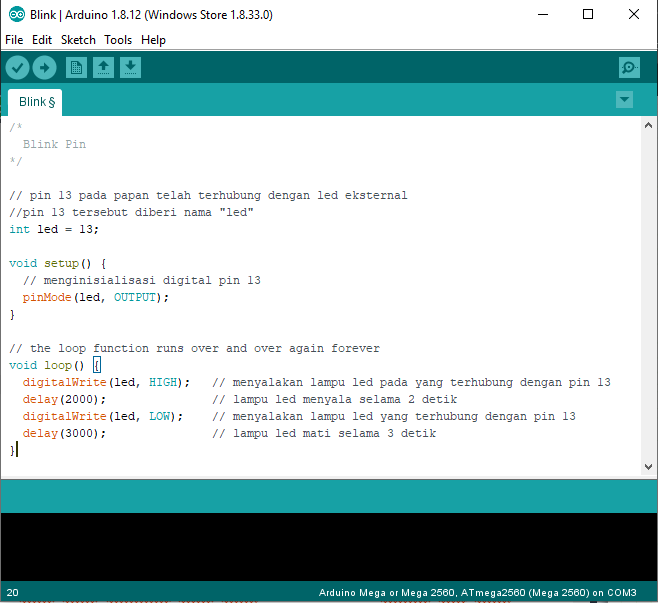
\includegraphics[scale=0.75]{blink_test_pin.png}  
        	\caption[\textit{Blink Test Pin}]{\textit{Blink Test Pin}}
        	\label{fig:Blink Test Pin} 
        \end{figure}
    
\end{itemize}



\section{Raspberry}
Raspberry merupakan komputer berukuran kecil yang dapat terhubung dengan desktop ataupun \textit{notebook}. Penggunaan sistem operasi linux oleh Raspberry, memungkinkan pengguna untuk mengerjakan proyek dan bereksperimen dengan sistem operasi yang bersifat \textit{open-source}. Raspberry juga dapat bertindak sebagai SINK (\textit{base station}), yang bertujuan untuk meneruskan data yang dikirimkan oleh node sensor ke server\cite{ahmad:17:raspberry}.

\subsection{Jenis-jenis Raspberry} \label{Jenis Raspberry}
Sama dengan perangkat keras arduino, Raspberry memiliki beberapa model dengan spesifikasi yang berbeda-beda. Pada umumnya perangkat keras ini menggunakan SoC (System on Chip) ARM 64-bit dan dilengkapi dengan RAM sebesar 512MB. Beberapa model Raspberry antara lain: 
\begin{itemize}
    \item Raspberry pi A
    
    Raspberry pi A, merupakan perangkat keras generasi pertama yang hanya memiliki sebuah USB port dan SDRAM sebesar 256MB. Perangkat keras ini juga dilengkapi dengan processor ARM 11. Jumlah USB Port yang sedikit memungkinkan penggunaan konsumsi daya yang lebih kecil dibanding model Raspberry lainnya.
    
    \begin{figure}[H]
    	\centering  
    	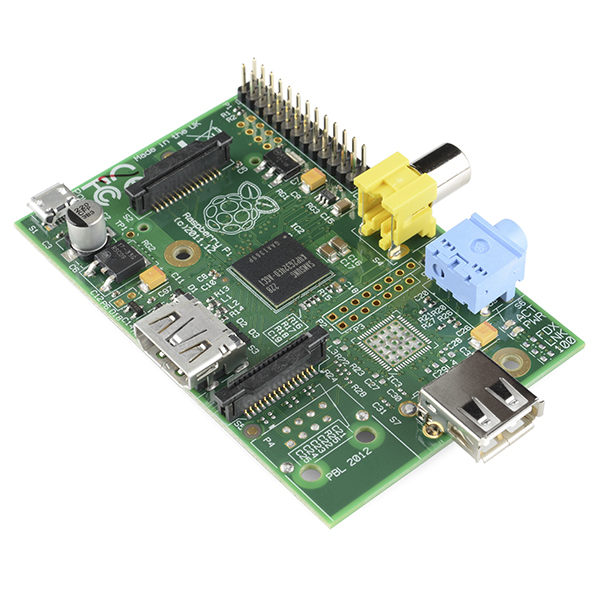
\includegraphics[scale=1]{raps-a.jpg}  
    	\caption[Raspberry pi A]{Raspberry pi A} 
    	\label{fig:Raspberry pi A} 
    \end{figure}
    
    \item Raspberry pi A+
    
    Pengembangan yang dilakukan pada Raspberry pi A, memunculkan perangkat keras model baru dengan nama Raspberry pi A+. Raspberry pi A+ memiliki spesifikasi yang mirip dengan Raspberry pi A. Namun, Raspberry A+ memiliki ukuran yang lebih kecil dibandingkan model lainnya, yaitu hanya 65mm saja.
    
    \begin{figure}[H]
    	\centering  
    	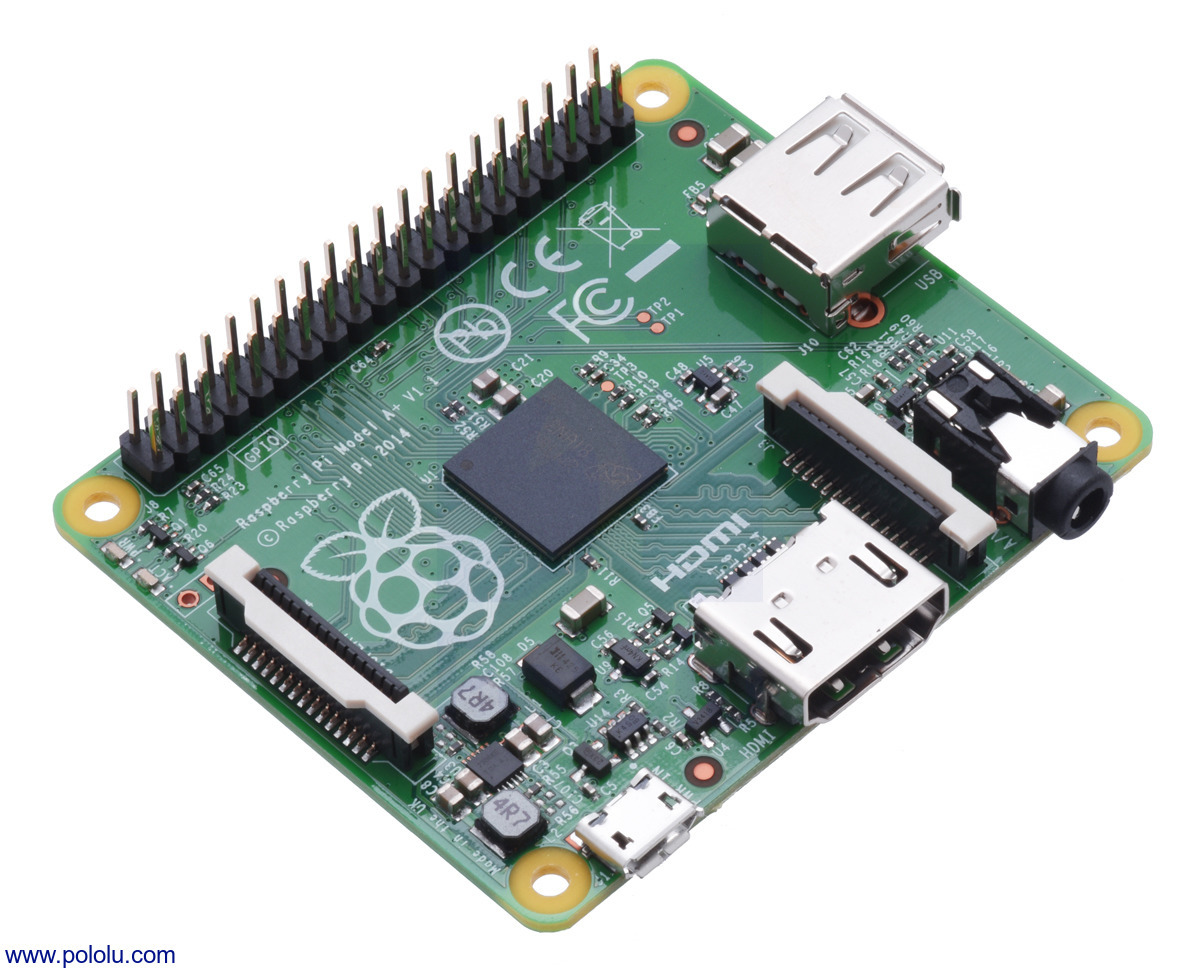
\includegraphics[scale=0.18]{raps-a+.png}  
    	\caption[Raspberry pi A+]{Raspberry pi A+} 
    	\label{fig:Raspberry pi A+} 
    \end{figure}
     
    \item Raspberry pi B
    
    Pada Raspberry pi B, terjadi penambahan di berbagai spesfikasi. Kapasitas RAM pada perangkat keras ini lebih besar dibanding generasi sebelumnya yang hanya 256MB, begitupula dengan jumlah port yang dimilikinya. Kapasitas RAM yang dimiliki Raspberry pi B adalah sebesar 521MB dan memiliki dua buah port USB. Raspberry pi B juga telah dilengkapi dengan sebuah ethernet, yang merupakan salah satu dari dua port USB yang disebutkan.
    
    \begin{figure}[H]
    	\centering  
    	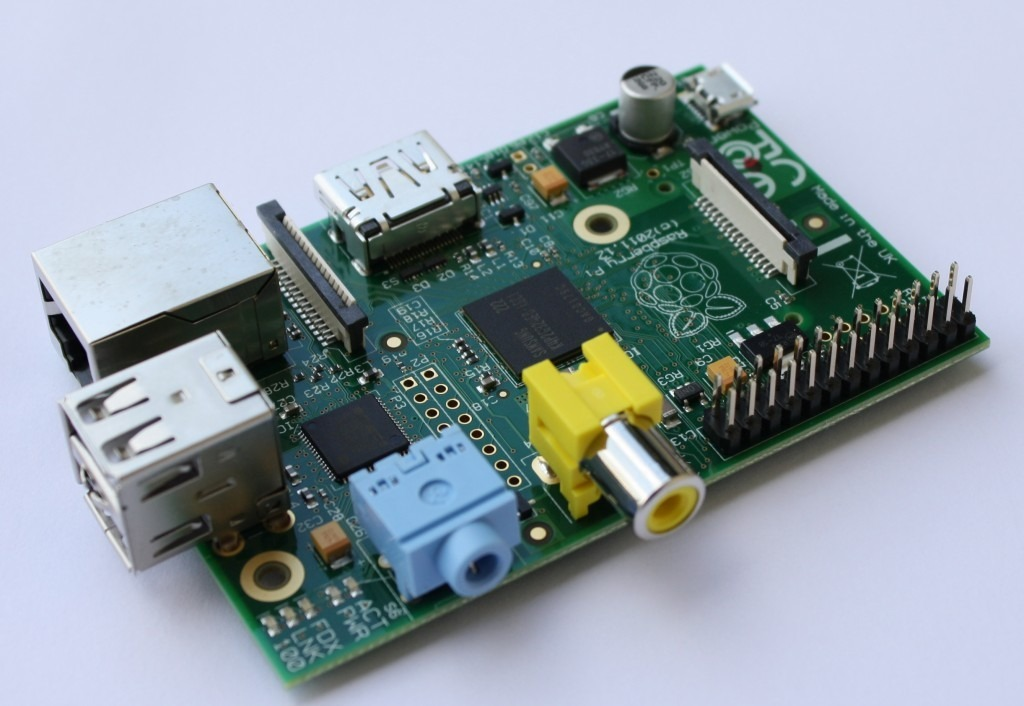
\includegraphics[scale=0.17]{raps-b.jpg}  
    	\caption[Raspberry pi B]{Raspberry pi B} 
    	\label{fig:Raspberry pi B} 
    \end{figure}
    
    \item Raspberry pi B+
    
     Raspberry pi B+ merupakan pengembangan dari model sebelumnya, Raspberry pi B. Namun, konsumsi daya yang digunakan lebih kecil dibanding model sebelumnya.
     
     \begin{figure}[H]
    	\centering  
    	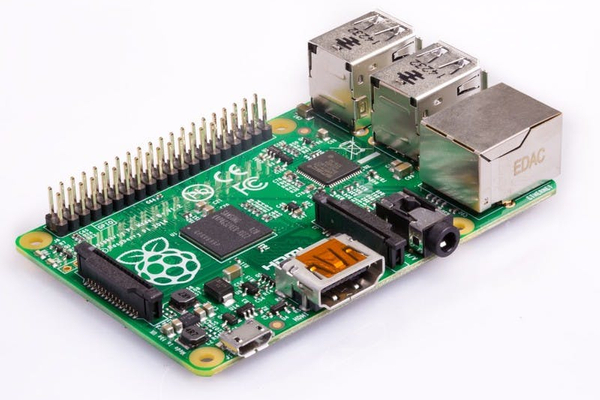
\includegraphics[scale=0.3]{raps-b+.jpg}  
    	\caption[Raspberry pi B+]{Raspberry pi B+} 
    	\label{fig:Raspberry pi B+} 
    \end{figure}
    
    \item Raspberry pi 2 B+
    
    Model Raspberry pi 2 B+ memungkinkan pengguna untuk menjalankan banyak distribusi sistem operasi. Hal ini dikarenakan model ini telah menggunakan processor dengan jenis ARMv7.
    
    \begin{figure}[H]
    	\centering  
    	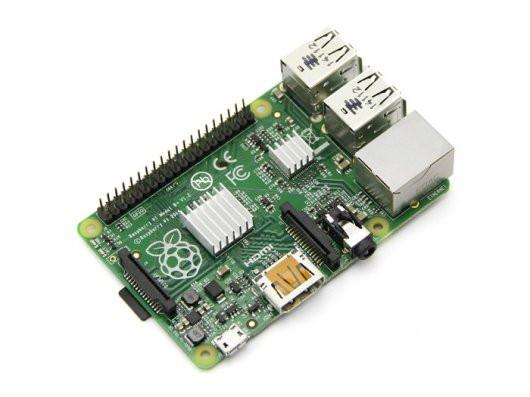
\includegraphics[scale=0.4]{raps-2-b+.jpg}  
    	\caption[Raspberry pi 2 B+]{Raspberry pi 2 B+} 
    	\label{fig:Raspberry pi 2 B+} 
    \end{figure}
    
    \item Raspberry pi 3 B+
    
    Model Raspberry pi 3 B+, telah terintergrasi dengan Bluetooth 4.1 dan Bluetooth Low Energy(BLE). Dengan memanfaatkan teknologi bluetooth, pengguna tidak lagi memerlukan modul USB wireless LAN tambahan, dalam perangkat keras Raspberry pi 3 B+.
    
    \begin{figure}[H]
    	\centering  
    	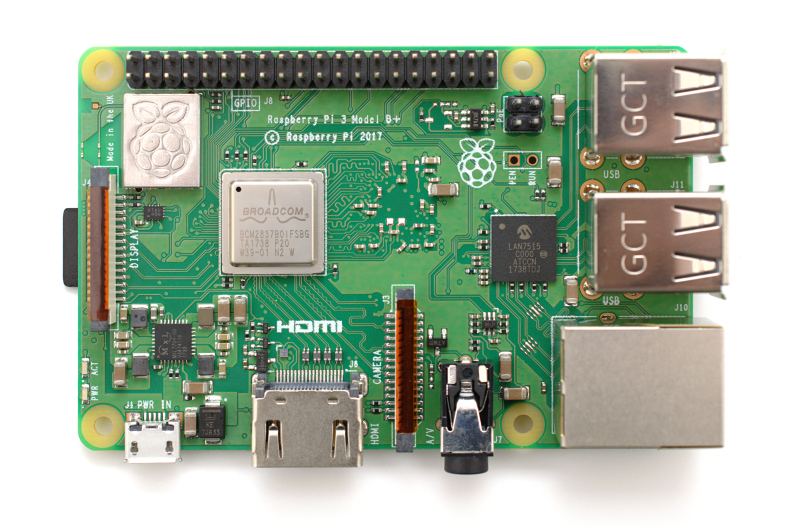
\includegraphics[scale=0.20]{raps-3-b+.png}  
    	\caption[Raspberry pi 3 B+]{Raspberry pi 3 B+} 
    	\label{fig:Raspberry pi 3 B+} 
    \end{figure}
\end{itemize}

\subsection{Pemrograman Raspberry}
Saat ini sudah banyak bahasa pemrograman yang telah disesuaikan untuk Raspberry pi, seperti bahasa pemrograman Python, C, C ++, Java, Scratch, dan Ruby. Semua bahasa pemrograman tersebut telah terinstall secara default pada Raspberry pi, dan siap digunakan oleh pengguna sesuai dengan bahasa pilihannya masing-masing.

\subsection{Pemrograman Python untuk Raspberry}
Salah satu contoh pemrograman di Raspberry menggunakan bahasa pemrograman python adalah mengubah nama \textit{host} menjadi \textit{ip address}. Pada IDE / Python Shell masukan kode seperti yang terdapat pada kode program \ref{Test Pyhton Rapsberry}. Program akan mencari alamat ip dari nama website yang terdapat dalam variabel website. Program dapat dijalankan dengan menekan tombol 'Run Module' pada menu 'Run' atau menekan key 'F5' pada keyboard. Ketika module dijalankan maka akan tampil Python Shell yang merupakan hasil pengolahan kode program yang dieksekusi, seperti yang ditunjukan pada Gambar~\ref{fig:Shell Python setelah eksekusi module}. 

    % \begin{figure}[H]
    % 	\centering  
    % 	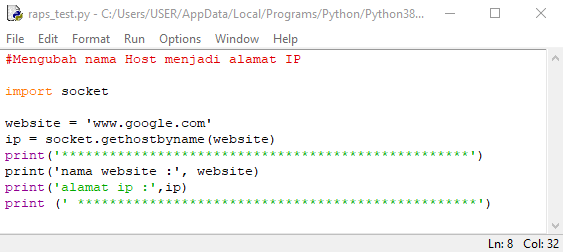
\includegraphics[scale=0.85]{raps_test_code.png}  
    % 	\caption[Pemrograman Python untuk Raspberry]{Pemrograman Python untuk Raspberry} 
    % 	\label{fig:Pemrograman Python pada Raspberry} 
    % \end{figure}
    
    \begin{lstlisting}[language=Python, caption=rasp\_test.py,label=Test Pyhton Rapsberry]
    #Mengubah nama Host menjadi alamat IP
    
    import socket
    
    website = 'www.google.com'
    ip = socket.gethostbyname (website)
    print('*************************')
    print('nama website :', website)
    print('alamat ip :', ip)
    print('*************************')
    \end{lstlisting}
    
    \begin{figure}[H]
    	\centering  
    	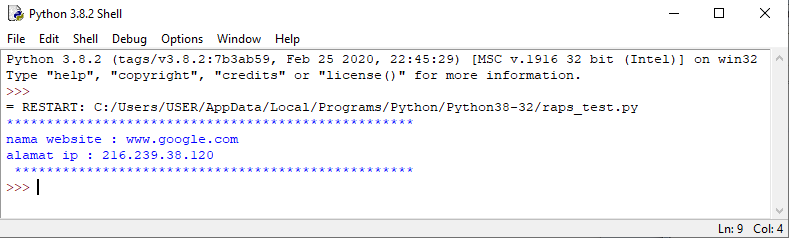
\includegraphics[scale=0.75]{raps_test_shell.png}  
    	\caption[Shell python setelah eksekusi \textit{module}]{Shell Python setelah eksekusi \textit{module}} 
    	\label{fig:Shell Python setelah eksekusi module} 
    \end{figure}

\section{Basis Data}
Basis  data  adalah  kumpulan  informasi  yang  disimpan  di dalam  komputer  secara  sistematik  sehingga  dapat  diperiksa menggunakan  suatu  program  komputer  untuk  memperoleh informasi dari basis data tersebut. Pada tahun 1960 Charles Bachman merancang \textit{Database Management System} (DBMS) yang digunakan untuk menyimpan data. Kemudian pada tahun yang sama, \textit{International Business Machines   Corporation} (IBM)  mengembangkan  sistem  manajemen  informasi DBMS. Terdapat  beberapa  jenis  bahasa  komputer  yang  digunakan  saat membangun  dan  memanipulasi  sebuah  basis  data,  yaitu Data \textit{Definition  Language} (DDL), \textit{Data  Manipulation  Language} (DML), dan \textit{Data Control Language} (DCL).
\textit{Entity   Relation   Diagram} atau   ERD   adalah   suatu model  untuk  menjelaskan  hubungan  antar  data  dalam basis   data   berdasarkan   objek-objek   dasar   data   yang mempunyai hubungan antar relasi. ERD juga digunakan untuk  memodelkan  struktur  data  dan  hubungan  antardata, dan menggambarkannya digunakan beberapa notasi dan simbol. 
    





% \section{Kutipan}
% \label{subs:kutipan} 
% Berikut contoh kutipan dari berbagai sumber, untuk keterangan lebih lengkap, silahkan membaca file referensi.bib yang disediakan juga di template ini.
% Contoh kutipan:
% \begin{itemize}
% 	\item Buku:~\cite{berg:08:compgeom} 
% 	\item Bab dalam buku:~\cite{kreveld:04:GIS}
% 	\item Artikel dari Jurnal:~\cite{buchin:13:median}
% 	\item Artikel dari prosiding seminar/konferensi:~\cite{kreveld:11:median}
% 	\item Skripsi/Thesis/Disertasi:~\cite{lionov:02:animasi}~\cite{wiratma:10:following}~\cite{wiratma:22:later}
% 	\item Technical/Scientific Report:~\cite{kreveld:07:watertight}
% 	\item RFC (Request For Comments):~\cite{RFC1654}
% 	\item Technical Documentation/Technical Manual:~\cite{Z.500}~\cite{unicode:16:stdv9}~\cite{google:16:and7}
% 	\item Paten:~\cite{webb:12:comm}
% 	\item Tidak dipublikasikan:~\cite{wiratma:09:median}~\cite{lionov:11:cpoly}
% 	\item Laman web:~\cite{erickson:03:cgmodel}  
% 	\item Lain-lain:~\cite{agung:12:tango}
% \end{itemize}    
  
% \subsection{Gambar}

% Pada hampir semua editor, penempatan gambar di dalam dokumen \LaTeX{} tidak dapat dilakukan melalui proses {\it drag and drop}.
% Perhatikan contoh pada file bab2.tex untuk melihat bagaimana cara menempatkan gambar.
% Beberapa hal yang harus diperhatikan pada saat menempatkan gambar:
% \begin{itemize}
% 	\item Setiap gambar {\bf harus} diacu di dalam teks (gunakan {\it field} {\sc label})
% 	\item {\it Field} {\sc caption} digunakan untuk teks pengantar pada gambar. Terdapat dua bagian yaitu yang ada di antara tanda $[$ dan $]$ dan yang ada di antara tanda $\{$ dan $\}$. Yang pertama akan muncul di Daftar Gambar, sedangkan yang kedua akan muncul di teks pengantar gambar. Untuk skripsi ini, samakan isi keduanya.
% 	\item Jenis file yang dapat digunakan sebagai gambar cukup banyak, tetapi yang paling populer adalah tipe {\sc png} (lihat Gambar~\ref{fig:ularpng}), tipe {\sc jpg} (Gambar~\ref{fig:ularjpg}) dan tipe {\sc pdf} (Gambar~\ref{fig:ularpdf})
% 	\item Besarnya gambar dapat diatur dengan {\it field} {\sc scale}.
% 	\item Penempatan gambar diatur menggunakan {\it placement specifier} (di antara tanda  $[$ dan $]$ setelah deklarasi gambar.
% 	Yang umum digunakan adalah {\bf H} untuk menempatkan gambar {\bf sesuai} penempatannya di file .tex atau  {\bf h} yang berarti "kira-kira" di sini. \\
% 	Jika tidak menggunakan {\it placement specifier}, \LaTeX{} akan menempatkan gambar secara otomatis untuk menghindari bagian kosong pada dokumen anda.
% 	Walaupun cara ini sangat mudah, hindarkan terjadinya penempatan dua gambar secara berurutan. 	
% 	\begin{itemize}
% 		\item Gambar~\ref{fig:ularpng} ditempatkan di bagian atas halaman, walaupun penempatannya dilakukan setelah penulisan 3 paragraf setelah penjelasan ini.
% 		\item Gambar~\ref{fig:ularjpg} dengan skala 0.5 ditempatkan di antara dua buah paragraf. Perhatikan penulisannya di dalam file bab2.tex!
% 		\item Gambar~\ref{fig:ularpdf} ditempatkan menggunakan {\it specifier} {\bf h}.
% 	\end{itemize}
% \end{itemize}
 
% \dtext{17-18}
% \begin{figure} 
% 	\centering  
% 	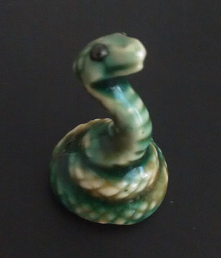
\includegraphics[scale=1]{ular-png}  
% 	\caption[Gambar {\it Serpentes} dalam format png]{Gambar {\it Serpentes} dalam format png} 
% 	\label{fig:ularpng} 
% \end{figure} 

% \dtext{19-20}
% \begin{figure}[H]
% 	\centering  
% 	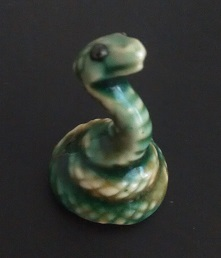
\includegraphics[scale=0.5]{ular-jpg}  
% 	\caption[Ular kecil]{Ular kecil} 
% 	\label{fig:ularjpg} 
% \end{figure} 
% \dtext{21-22}

% \begin{figure}[ht] 
% 	\centering  
% 	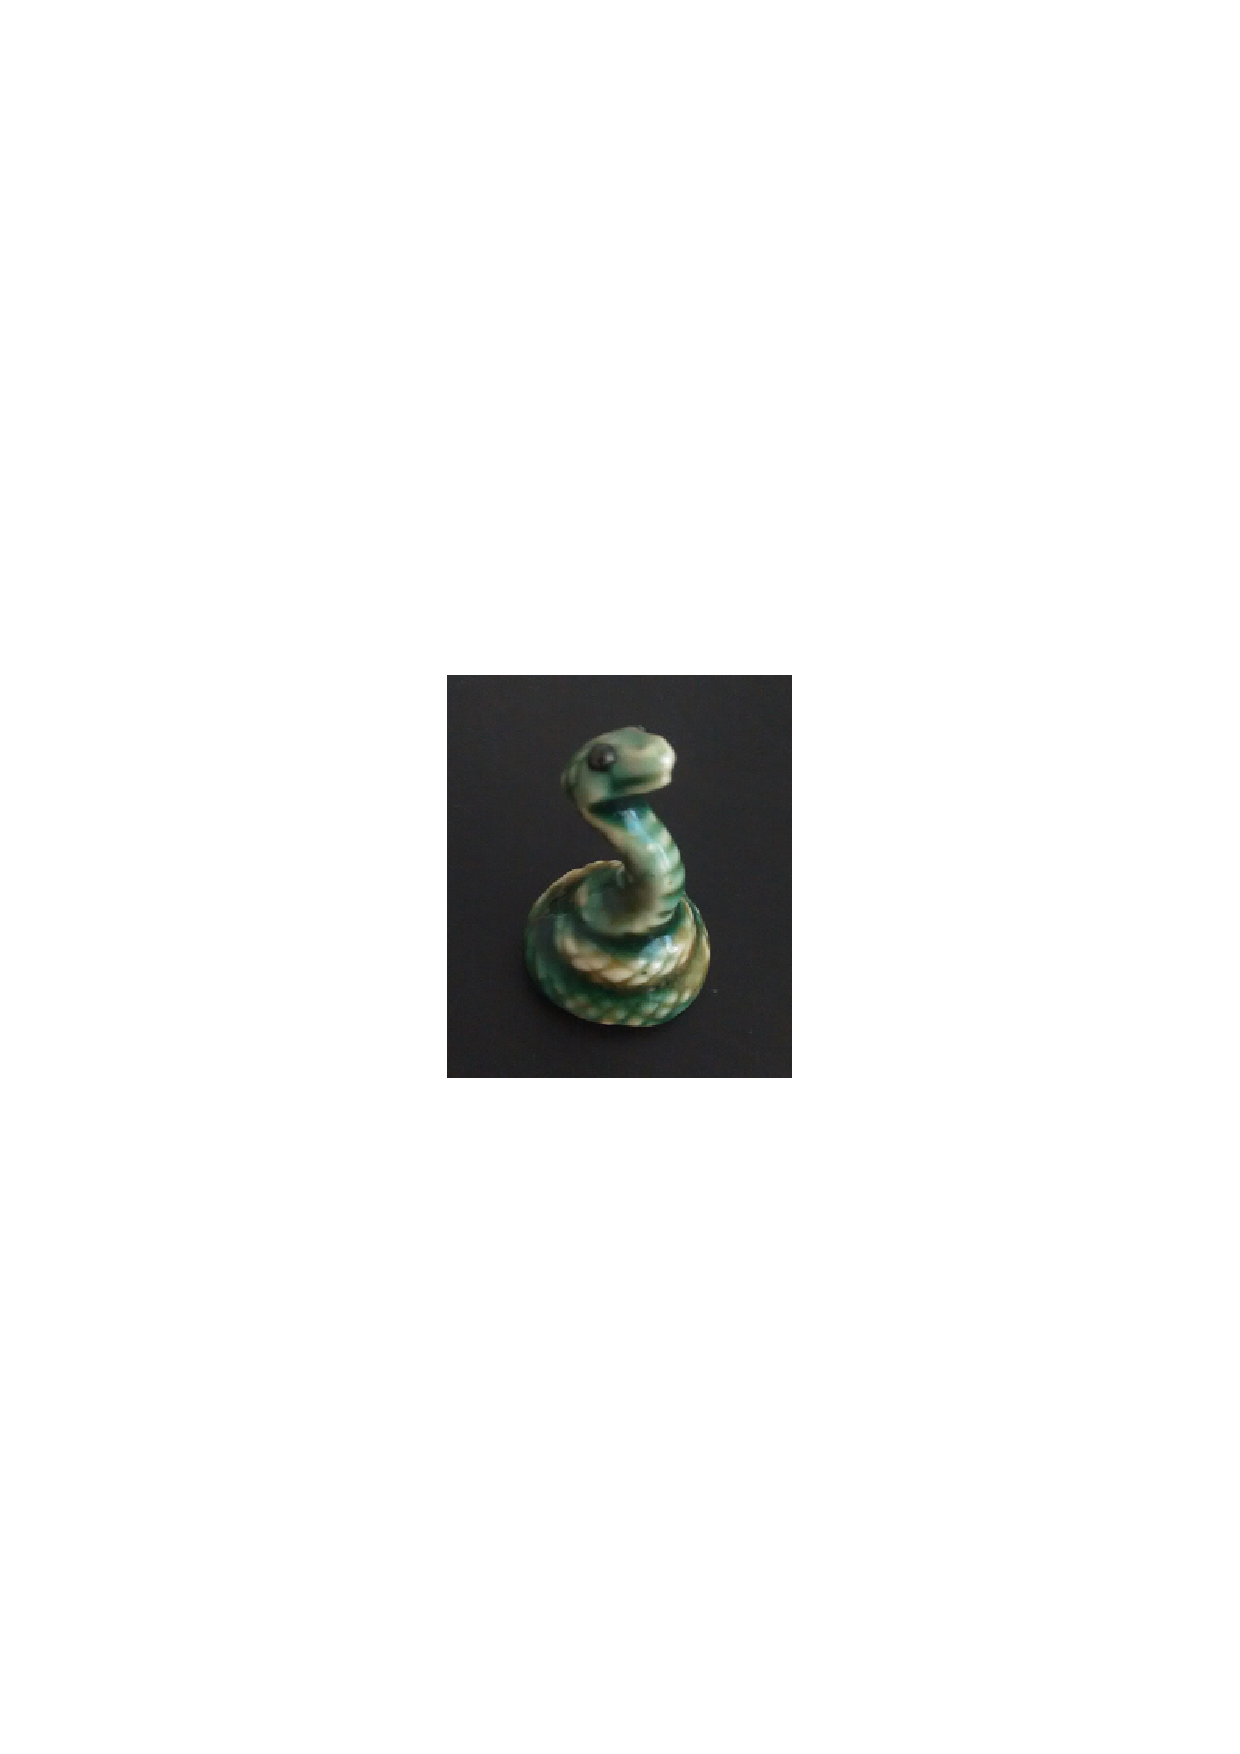
\includegraphics[scale=1]{ular-pdf}  
% 	\caption[ {\it Serpentes} betina]{ {\it Serpentes} jantan} 
% 	\label{fig:ularpdf} 
% \end{figure} 
 
